\section{Induction machines}

%%%%%%%%%%%%%%%%%%%%%%%%%%%%%%%%%%%%%%%%%%%%%%%%%%%%%%%%%%%%%
\subsection{Operation principle}
%%%%%%%%%%%%%%%%%%%%%%%%%%%%%%%%%%%%%%%%%%%%%%%%%%%%%%%%%%%%%

%%%%%%%%%%%%%%%%%%%%%%%%%%%%%%%%%%%%%%%%%%%%%%%%%%%%%%%%%%%%%
%% Basic induction machine (IM) representation %%
%%%%%%%%%%%%%%%%%%%%%%%%%%%%%%%%%%%%%%%%%%%%%%%%%%%%%%%%%%%%%
\begin{frame}
	\frametitle{Basic induction machine (IM) representation}
    \begin{columns}
		\begin{column}{0.55\textwidth}
	       \begin{itemize}
            \item Three-phase stator + three-phase rotor: ``rotating three-phase transformer''\newline (plus air gap)
            \item Rotor angular speed: $\omega_\mathrm{r}$
            \item Rotor angular displacement: $\varepsilon_\mathrm{r}$
            \item Index ``s'' for stator, ``r'' for rotor quantities
           \end{itemize}
           \onslide<2->{
           \begin{varblock}{Fundamental wave model}
              While the previous chapter has revealed that the magnetic flux distribution in the air gap is subject to plentiful harmonics, the following model limits itself to the fundamental wave.
           \end{varblock}}
        \end{column}
        \begin{column}{0.45\textwidth}
            \begin{figure}
                \centering
                \includegraphics[width=0.85\textwidth]{fig/lec06/Simple_three_phase_induction_machine_lumped_coils.pdf}
                \caption{Elementary three-phase induction machine (IM) lumped-coil representation ($p=1$ pole pair)}
                \label{fig:Simple_three_phase_induction_machine_lumped_coils}
            \end{figure}
        \end{column}
    \end{columns}
\end{frame}

%%%%%%%%%%%%%%%%%%%%%%%%%%%%%%%%%%%%%%%%%%%%%%%%%%%%%%%%%%%%%
%% Visualization of the asynchronous IM operation %%
%%%%%%%%%%%%%%%%%%%%%%%%%%%%%%%%%%%%%%%%%%%%%%%%%%%%%%%%%%%%%
\begin{frame}
	\frametitle{Visualization of the asynchronous IM operation}
    \begin{figure}
        \centering
        \movie{\includegraphics[height=0.85\textheight]{fig/lec06/IM_slip_0_load_angle_90_preview.png}}{fig/lec06/IM_slip_0_load_angle_90_animation.gif}
        \vspace{-0.25cm}
        \caption{Exemplary IM operation at $\omega=2 \pi \SI{50}{\per\second}$ in motoric operation (positive average torque)}
        \label{fig:IM_slip_0_load_angle_90_animation}
    \end{figure}
\end{frame}

%%%%%%%%%%%%%%%%%%%%%%%%%%%%%%%%%%%%%%%%%%%%%%%%%%%%%%%%%%%%%
%% Visualization of the asynchronous IM operation (cont.) %%
%%%%%%%%%%%%%%%%%%%%%%%%%%%%%%%%%%%%%%%%%%%%%%%%%%%%%%%%%%%%%
\begin{frame}
	\frametitle{Visualization of the asynchronous IM operation (cont.)}
    \begin{figure}
        \centering
        \movie{\includegraphics[height=0.85\textheight]{fig/lec06/IM_slip_0_load_angle_0_preview.png}}{fig/lec06/IM_slip_0_load_angle_0_animation.gif}
        \vspace{-0.25cm}
        \caption{Exemplary IM operation at $\omega=2 \pi \SI{50}{\per\second}$ in no-load operation (zero average torque)}
        \label{fig:IM_slip_0_load_angle_0_animation}
    \end{figure}
\end{frame}

%%%%%%%%%%%%%%%%%%%%%%%%%%%%%%%%%%%%%%%%%%%%%%%%%%%%%%%%%%%%%
\subsection{Model in stationary three-phase coordinates}
%%%%%%%%%%%%%%%%%%%%%%%%%%%%%%%%%%%%%%%%%%%%%%%%%%%%%%%%%%%%%

%%%%%%%%%%%%%%%%%%%%%%%%%%%%%%%%%%%%%%%%%%%%%%%%%%%%%%%%%%%%%
%% Dynamical IM model %%
%%%%%%%%%%%%%%%%%%%%%%%%%%%%%%%%%%%%%%%%%%%%%%%%%%%%%%%%%%%%%
\begin{frame}
	\frametitle{Dynamical IM model}
    Based on Faraday's and Ohm's laws, we can write the following equations for the stator 
    \begin{equation}
            \bm{u}^\mathrm{s}_\mathrm{s,abc}(t) = R_\mathrm{s}\bm{i}^\mathrm{s}_\mathrm{s,abc}(t)+\frac{\mathrm{d}}{\mathrm{d}t}\bm{\psi}^\mathrm{s}_\mathrm{s,abc}(t) \hspace{0.2cm} \Leftrightarrow \hspace{0.2cm} \begin{bmatrix}
                u_{\mathrm{s,a}}^\mathrm{s}(t)\\
                u_{\mathrm{s,b}}^\mathrm{s}(t)\\
                u_{\mathrm{s,c}}(t)\\
            \end{bmatrix} = R_\mathrm{s} \begin{bmatrix}
                i_{\mathrm{s,a}}^\mathrm{s}(t)\\
                i_{\mathrm{s,b}}^\mathrm{s}(t)\\
                i_{\mathrm{s,c}}^\mathrm{s}(t)\\
            \end{bmatrix} + \frac{\mathrm{d}}{\mathrm{d}t} \begin{bmatrix}
                \psi_{\mathrm{s,a}}^\mathrm{s}(t)\\
                \psi_{\mathrm{s,b}}^\mathrm{s}(t)\\
                \psi_{\mathrm{s,c}}^\mathrm{s}(t)\\
            \end{bmatrix}
            \label{eq:IM_stator_three_phase_voltage_equation}
    \end{equation}
    \pause
    and rotor
    \begin{equation}
            \bm{u}^\mathrm{r}_\mathrm{r,abc}(t) = R_\mathrm{r}\bm{i}^\mathrm{r}_\mathrm{r,abc}(t)+\frac{\mathrm{d}}{\mathrm{d}t}\bm{\psi}^\mathrm{r}_\mathrm{r,abc}(t) \hspace{0.2cm} \Leftrightarrow \hspace{0.2cm} \begin{bmatrix}
                u_{\mathrm{r,a}}^\mathrm{r}(t)\\
                u_{\mathrm{r,b}}^\mathrm{r}(t)\\
                u_{\mathrm{r,c}}^\mathrm{r}(t)\\
            \end{bmatrix} = R_\mathrm{r} \begin{bmatrix}
                i_{\mathrm{r,a}}^\mathrm{r}(t)\\
                i_{\mathrm{r,b}}^\mathrm{r}(t)\\
                i_{\mathrm{r,c}}^\mathrm{r}(t)\\
            \end{bmatrix} + \frac{\mathrm{d}}{\mathrm{d}t} \begin{bmatrix}
                \psi_{\mathrm{r,a}}^\mathrm{r}(t)\\
                \psi_{\mathrm{r,b}}^\mathrm{r}(t)\\
                \psi_{\mathrm{r,c}}^\mathrm{r}(t)\\
            \end{bmatrix}
            \label{eq:IM_rotor_three_phase_voltage_equation}
    \end{equation}
which are generally applicable as only identical resistances per phase on the stator and rotor are assumed. \pause Above, the lower index denotes the physical location of the quantities, while the upper index indicates the coordinate system orientation.
\end{frame}

%%%%%%%%%%%%%%%%%%%%%%%%%%%%%%%%%%%%%%%%%%%%%%%%%%%%%%%%%%%%%
%% Flux linakge model %%
%%%%%%%%%%%%%%%%%%%%%%%%%%%%%%%%%%%%%%%%%%%%%%%%%%%%%%%%%%%%%
\begin{frame}
	\frametitle{Flux linkage model}
    \onslide<2->
    \begin{columns}
		\begin{column}{0.55\textwidth}
            In contrast to the simple three-phase transformer model \eqref{eq:Three_phase_transformer_flux_linkage}, the flux linkage model of the IM is more complex: 
	       \begin{itemize}
            \item<2-> Due to the spatial 120$^\circ$ phase shift between the windings of the stator and rotor, the abc phases are all mutually coupled. 
            \item<3-> The flux paths and physical dimensions of the stator and rotor are not identical, i.e., the rotor and stator inductances are different (even if the winding turns $N_\mathrm{s}$ and $N_\mathrm{r}$ are identical). 
            \item<4-> The coupling between the stator and rotor is rotor position-dependent (not explicitly shown on the right due to space limitations). 
           \end{itemize}
        \end{column}
        \begin{column}{0.45\textwidth}
            \onslide<1->
                \begin{figure}
                    \centering
                    \includegraphics[width=0.75\textwidth]{fig/lec06/Inductive_coupling_stator_rotor.pdf}
                    \caption{Simplified representation of the inductive coupling between the stator/rotor phases of the IM}
                    \label{fig:Inductive_coupling_stator_rotor_IM}
                \end{figure}
            
        \end{column}
    \end{columns}
\end{frame}

%%%%%%%%%%%%%%%%%%%%%%%%%%%%%%%%%%%%%%%%%%%%%%%%%%%%%%%%%%%%%
%% Flux linakge model %%
%%%%%%%%%%%%%%%%%%%%%%%%%%%%%%%%%%%%%%%%%%%%%%%%%%%%%%%%%%%%%
\begin{frame}
	\frametitle{Flux linkages of the three-phase model}
    \onslide<1->
    Based on the previous considerations, the flux linkages are given by
    \begin{equation}
        \renewcommand*{\arraystretch}{1.15}
        \begin{split}
            \uncover<+->{
            \bm{\psi}^\mathrm{s}_\mathrm{s,abc}(t) &=\begin{bmatrix}
                L_\mathrm{s} & -\frac{M_\mathrm{s}}{2} & -\frac{M_\mathrm{s}}{2}\\
                -\frac{M_\mathrm{s}}{2} & L_\mathrm{s} & -\frac{M_\mathrm{s}}{2}\\
                -\frac{M_\mathrm{s}}{2} & -\frac{M_\mathrm{s}}{2} & L_\mathrm{s}
            \end{bmatrix} \bm{i}^\mathrm{s}_\mathrm{s,abc}(t)}\uncover<+->{ +  M_{\mathrm{r}}\frac{N_\mathrm{s}}{N_\mathrm{r}} \bm{\mathcal{R}}_\mathrm{abc}(\varepsilon_\mathrm{r,el}(t))\bm{i}^\mathrm{r}_\mathrm{r,abc}(t),}\\
            \uncover<+->{
            \bm{\psi}^\mathrm{r}_\mathrm{r,abc}(t) &= \begin{bmatrix}
                L_\mathrm{r} & -\frac{M_\mathrm{r}}{2} & -\frac{M_\mathrm{r}}{2}\\
                -\frac{M_\mathrm{r}}{2} & L_\mathrm{r} & -\frac{M_\mathrm{r}}{2}\\
                -\frac{M_\mathrm{r}}{2} & -\frac{M_\mathrm{r}}{2} & L_\mathrm{r}
            \end{bmatrix} \bm{i}^\mathrm{r}_\mathrm{r,abc}(t) +  M_{\mathrm{s}}\frac{N_\mathrm{r}}{N_\mathrm{s}} \bm{\mathcal{R}}_\mathrm{abc}(\varepsilon_\mathrm{r,el}(t))\T\bm{i}^\mathrm{s}_\mathrm{s,abc}(t)}
        \end{split}
        \label{eq:Flux_linkage_model_IM_abc}
    \end{equation}
    \onslide<+->
    with $\varepsilon_\mathrm{r,el}(t)=p\varepsilon_\mathrm{r}(t)$ and the transformation matrix
    \begin{equation}
        \renewcommand*{\arraystretch}{1.15}
        \bm{\mathcal{R}}_\mathrm{abc}(\varepsilon_\mathrm{r,el}(t)) =\begin{bmatrix}
           \cos(\varepsilon_\mathrm{r,el}(t))  & \cos(\varepsilon_\mathrm{r,el}(t) + \frac{2\pi}{3}) & \cos(\varepsilon_\mathrm{r,el}(t) - \frac{2\pi}{3})\\
            \cos(\varepsilon_\mathrm{r,el}(t) - \frac{2\pi}{3}) & \cos(\varepsilon_\mathrm{r,el}(t)) & \cos(\varepsilon_\mathrm{r,el}(t) + \frac{2\pi}{3})\\
            \cos(\varepsilon_\mathrm{r,el}(t) + \frac{2\pi}{3}) & \cos(\varepsilon_\mathrm{r,el}(t) - \frac{2\pi}{3}) & \cos(\varepsilon_\mathrm{r,el}(t))
        \end{bmatrix}.
    \end{equation}
\end{frame}

%%%%%%%%%%%%%%%%%%%%%%%%%%%%%%%%%%%%%%%%%%%%%%%%%%%%%%%%%%%%%
%% \frametitle{Inductance matrices} %%
%%%%%%%%%%%%%%%%%%%%%%%%%%%%%%%%%%%%%%%%%%%%%%%%%%%%%%%%%%%%%
\begin{frame}
	\frametitle{Inductance matrices of the three-phase model}
    The inductance matrices
    $$\renewcommand*{\arraystretch}{1.15} 
    \bm{L}_\mathrm{s,abc} = \begin{bmatrix}
        L_\mathrm{s} & -\frac{M_\mathrm{s}}{2} & -\frac{M_\mathrm{s}}{2}\\
        -\frac{M_\mathrm{s}}{2} & L_\mathrm{s} & -\frac{M_\mathrm{s}}{2}\\
        -\frac{M_\mathrm{s}}{2} & -\frac{M_\mathrm{s}}{2} & L_\mathrm{s}
    \end{bmatrix}, \qquad  \bm{L}_\mathrm{r,abc} = \begin{bmatrix}
        L_\mathrm{r} & -\frac{M_\mathrm{r}}{2} & -\frac{M_\mathrm{r}}{2}\\
        -\frac{M_\mathrm{r}}{2} & L_\mathrm{r} & -\frac{M_\mathrm{r}}{2}\\
        -\frac{M_\mathrm{r}}{2} & -\frac{M_\mathrm{r}}{2} & L_\mathrm{r}
    \end{bmatrix}$$
    are based on the following considerations. 
    \begin{itemize}
        \item The self-inductances cover both the leakage and mutual coupling to other windings: $L_\mathrm{s/r}=L_\mathrm{s/r, \sigma} + M_\mathrm{s/r}$.
        \item<2-> The mutual inductances on the stator/rotor $M_\mathrm{s/r}$ are identical, as all three phases share the same magnetic paths and have the same winding turns $N_\mathrm{s/r}$.
        \item<3-> The mutual inductances on the off diagonal represent the spatial displacement of the stator/rotor coils by $\pm 120^\circ$, which is why they are multiplied by $\cos(\pm 120^\circ)=-0.5$.
        \item<4-> In \eqref{eq:Flux_linkage_model_IM_abc}, the coupling term between stator and rotor is multiplied by the turn ratio to account for the different winding turns $N_\mathrm{s/r}$ (i.e., mapping the mutual inductances between stator/rotor).
    \end{itemize}
\end{frame}

%%%%%%%%%%%%%%%%%%%%%%%%%%%%%%%%%%%%%%%%%%%%%%%%%%%%%%%%%%%%%
\subsection{Model in stationary alpha-beta coordinates}
%%%%%%%%%%%%%%%%%%%%%%%%%%%%%%%%%%%%%%%%%%%%%%%%%%%%%%%%%%%%%

%%%%%%%%%%%%%%%%%%%%%%%%%%%%%%%%%%%%%%%%%%%%%%%%%%%%%%%%%%%%%
%% Orthogonal representation: alpha-beta coordinates %%
%%%%%%%%%%%%%%%%%%%%%%%%%%%%%%%%%%%%%%%%%%%%%%%%%%%%%%%%%%%%%
\begin{frame}
	\frametitle{Orthogonal representation: alpha-beta coordinates}
    \begin{columns}
		\begin{column}{0.55\textwidth}
	       \begin{itemize}
            \item<1-> The three-phase IM model is obviously quite unhandy: six differential equations plus a rather complicated magnetic circuit representation.
            \item<2-> Remedy: transform the three-phase model into the orthogonal $\alpha\beta$ coordinates.
            \item<3-> Advantage: only four differential equations and a simpler magnetic circuit representation (as one will see on the next slides).
           \end{itemize}
           \vspace{-0.4cm}
           \onslide<4->
           \begin{varblock}{Coordinate transformations}
              The following transformations of the IM model into different coordinate systems are pure mathematical ``tricks'' to simplify the analysis. The IM remains a three-phase machine. 
           \end{varblock}
        \end{column}
        \begin{column}{0.45\textwidth}
            \onslide<2->
            \begin{figure}
                \centering
                \includegraphics[width=0.85\textwidth]{fig/lec06/Induction_machine_alpha_beta.pdf}
                \caption{Conceptual IM representation within the orthogonal $\alpha\beta$ coordinates ($p=1$ pole pair)}
                \label{fig:Induction_machine_alpha_beta}
            \end{figure}
        \end{column}
    \end{columns}
\end{frame}

%%%%%%%%%%%%%%%%%%%%%%%%%%%%%%%%%%%%%%%%%%%%%%%%%%%%%%%%%%%%%
%% Clarke transformation %%
%%%%%%%%%%%%%%%%%%%%%%%%%%%%%%%%%%%%%%%%%%%%%%%%%%%%%%%%%%%%%
\begin{frame}
	\frametitle{Clarke transformation}
    To transform the three-phase model into the orthogonal $\alpha\beta$ coordinates, the Clarke transformation is applied. Consider any $\bm{x}_\mathrm{abc}\in\mathbb{R}^3$, then the Clarke transformation is given by
    \begin{equation}
        \renewcommand{\arraystretch}{1.2}
        \bm{x}_{\alpha \beta0} = \begin{bmatrix} x_\alpha \\ x_\beta \\ x_0\end{bmatrix} = \begin{bmatrix}
            \nicefrac{2}{3} & -\nicefrac{1}{3} & -\nicefrac{1}{3}\\
            0 & \nicefrac{1}{\sqrt{3}} & -\nicefrac{1}{\sqrt{3}}\\
            \nicefrac{\sqrt{2}}{3} & \nicefrac{\sqrt{2}}{3} & \nicefrac{\sqrt{2}}{3}
        \end{bmatrix} \begin{bmatrix} x_\mathrm{a} \\ x_\mathrm{b} \\ x_\mathrm{c}\end{bmatrix} = \bm{T}_\mathrm{c} \bm{x}_\mathrm{abc} 
        \label{eq:Clarke_transformation}
    \end{equation}
    \pause
    with the inverse transformation
    \begin{equation}
        \renewcommand{\arraystretch}{1.2}
        \bm{x}_\mathrm{abc}  = \begin{bmatrix}
            1 & 0 & \nicefrac{1}{\sqrt{2}}\\
            -\nicefrac{1}{2} & \nicefrac{\sqrt{3}}{2} & \nicefrac{1}{\sqrt{2}}\\
            -\nicefrac{1}{2} & -\nicefrac{\sqrt{3}}{2} & \nicefrac{1}{\sqrt{2}}
        \end{bmatrix} \begin{bmatrix} x_\alpha \\ x_\beta \\ x_0\end{bmatrix} = \bm{T}_\mathrm{c}^{-1} \bm{x}_{\alpha \beta 0}.
    \end{equation}
    \pause
    Above, $\bm{T}_\mathrm{c}\in\mathbb{R}^{3\times 3}$ is the Clarke transformation matrix and $\bm{x}_\mathrm{\alpha \beta0}\in\mathbb{R}^3$ the transformed vector.
\end{frame}

%%%%%%%%%%%%%%%%%%%%%%%%%%%%%%%%%%%%%%%%%%%%%%%%%%%%%%%%%%%%%
%% Clarke transformation: amplitude and power scaling %%
%%%%%%%%%%%%%%%%%%%%%%%%%%%%%%%%%%%%%%%%%%%%%%%%%%%%%%%%%%%%%
\begin{frame}
	\frametitle{Clarke transformation: amplitude and power scaling}
    The transformation \eqref{eq:Clarke_transformation} is amplitude-preserving, i.e., the amplitude of the $\alpha\beta$ vector is identical to the amplitude of the original abc vector. \pause On the other hand, the power is not preserved, as can be seen from the inner product of the transformed vectors (which commonly occurs in power calculations):
    \begin{equation*}
        \bm{x}_{\mathrm{abc}}\T \bm{y}_{\mathrm{abc}} = \bm{x}_\mathrm{\alpha \beta 0}\T\left(\bm{T}_\mathrm{c}^{-1}\right)\T \bm{T}_\mathrm{c}^{-1}\bm{y}_\mathrm{\alpha \beta 0} \quad \Leftrightarrow \quad x_\mathrm{a}y_\mathrm{a} + x_\mathrm{b}y_\mathrm{b} + x_\mathrm{c}y_\mathrm{c} = \frac{3}{2}\left(x_\alpha y_\alpha + x_\beta y_\beta + x_0 y_0 \right).
    \end{equation*}
    \pause
    The alternative power-preserving Clarke transformation variant is given by
    \begin{equation}
        \renewcommand{\arraystretch}{1.2}
        \bm{T}'_\mathrm{c} = \frac{\sqrt{3}}{2} \bm{T}_\mathrm{c} \qquad \left(\bm{T}'_\mathrm{c}\right)^{-1} = \left(\bm{T}'_\mathrm{c}\right)\T,
        \label{eq:Clarke_transformation_power_preserving}
    \end{equation}
    which utilizes an orthogonal transformation matrix. \pause However, when using $\bm{T}'_\mathrm{c}$ the amplitude of the transformed vector is not preserved. While being an arbitrary choice, we will stick to \eqref{eq:Clarke_transformation} as a convention for the following. 
\end{frame}

%%%%%%%%%%%%%%%%%%%%%%%%%%%%%%%%%%%%%%%%%%%%%%%%%%%%%%%%%%%%%
%% Clarke transformation: simplification for zero-component-free vectors %%
%%%%%%%%%%%%%%%%%%%%%%%%%%%%%%%%%%%%%%%%%%%%%%%%%%%%%%%%%%%%%
\begin{frame}
	\frametitle{Clarke transformation: simplification for zero-component-free vectors}
    If the abc vector $\bm{x}_\mathrm{abc}$ is zero-component-free, i.e.,  $$x_\mathrm{a} + x_\mathrm{b} +x_\mathrm{c} = 0,$$
    e.g., the phase currents of a star connected system, \pause the Clarke transformation simplifies to
    \begin{equation}
        \renewcommand{\arraystretch}{1.2}
        \bm{x}_{\alpha \beta} = \begin{bmatrix} x_\alpha \\ x_\beta \end{bmatrix} = \begin{bmatrix}
            \nicefrac{2}{3} & -\nicefrac{1}{3} & -\nicefrac{1}{3}\\
            0 & \nicefrac{1}{\sqrt{3}} & -\nicefrac{1}{\sqrt{3}}
        \end{bmatrix} \begin{bmatrix} x_\mathrm{a} \\ x_\mathrm{b} \\ x_\mathrm{c}\end{bmatrix} = \bm{T}_{23} \bm{x}_\mathrm{abc}
        \label{eq:Clarke_transformation_zero_component_free}
    \end{equation}
    \pause
    and
    \begin{equation}
        \renewcommand{\arraystretch}{1.2}
        \bm{x}_\mathrm{abc}  = \begin{bmatrix}
            1 & 0\\
            -\nicefrac{1}{2} & \nicefrac{\sqrt{3}}{2}\\
            -\nicefrac{1}{2} & -\nicefrac{\sqrt{3}}{2}
        \end{bmatrix} \begin{bmatrix} x_\alpha \\ x_\beta \end{bmatrix} = \bm{T}_{32} \bm{x}_{\alpha \beta}.
    \end{equation}     
\end{frame}

%%%%%%%%%%%%%%%%%%%%%%%%%%%%%%%%%%%%%%%%%%%%%%%%%%%%%%%%%%%%%
%% Clarke transformation: simplification for zero-component-free vectors %%
%%%%%%%%%%%%%%%%%%%%%%%%%%%%%%%%%%%%%%%%%%%%%%%%%%%%%%%%%%%%%
\begin{frame}
	\frametitle{Clarke transformation: simplification for zero-component-free vectors}
    \begin{figure}
        \centering
        \includegraphics[width=0.38\textwidth]{fig/lec06/abc_alphabeta_vectors.pdf}
        \caption{Geometrical interpretation of the Clarke
        transformation without zero components: mapping $\bm{x}_\mathrm{abc}\in\mathbb{R}^3$ to $\bm{x}_{\alpha\beta}\in\mathbb{R}^2$ without information loss (adapted from J.~B\"ocker, \textit{Controlled Three-Phase Drives}, Paderborn University, 2021)}
        \label{fig:abc_alphabeta_vectors}
    \end{figure}    
\end{frame}

%%%%%%%%%%%%%%%%%%%%%%%%%%%%%%%%%%%%%%%%%%%%%%%%%%%%%%%%%%%%%
%% IM model $\alpha\beta-\gamma\delta$ coordinates %%
%%%%%%%%%%%%%%%%%%%%%%%%%%%%%%%%%%%%%%%%%%%%%%%%%%%%%%%%%%%%%
\begin{frame}
	\frametitle{IM model $\alpha\beta$ coordinates}
    \onslide<+->
    Assuming zero-component-free three-phase quantities, multiplying the three-phase IM model \eqref{eq:IM_stator_three_phase_voltage_equation} and \eqref{eq:IM_rotor_three_phase_voltage_equation} with $\bm{T}_{23}$ results in
    \begin{equation}
        \begin{split}
        \uncover<+->{\bm{T}_{23}\bm{u}^\mathrm{s}_\mathrm{s,abc}(t) &= R_\mathrm{s} \bm{T}_{23}\bm{i}^\mathrm{s}_\mathrm{s,abc}(t)+ \bm{T}_{23}\frac{\mathrm{d}}{\mathrm{d}t}\bm{\psi}^\mathrm{s}_\mathrm{s,abc}(t)}\\
        \uncover<+->{\Leftrightarrow\quad \bm{u}^\mathrm{s}_\mathrm{s,\alpha\beta}(t) &= R_\mathrm{s} \bm{i}^\mathrm{s}_\mathrm{s,\alpha\beta}(t)+ \frac{\mathrm{d}}{\mathrm{d}t}\bm{\psi}^\mathrm{s}_\mathrm{s,\alpha\beta}(t)} 
    \end{split}
    \label{eq:IM_stator_alpha_beta_voltage_equation}
\end{equation}
\onslide<4->
{
and
}
\begin{equation}
    \begin{split}
        \uncover<+->{\bm{T}_{23}\bm{u}^\mathrm{r}_\mathrm{r,abc}(t) &= R_\mathrm{r} \bm{T}_{23}\bm{i}^\mathrm{r}_\mathrm{r,abc}(t)+ \bm{T}_{23}\frac{\mathrm{d}}{\mathrm{d}t}\bm{\psi}^\mathrm{r}_\mathrm{r,abc}(t)}\\
        \uncover<+->{\Leftrightarrow\quad  \bm{u}^\mathrm{r}_\mathrm{r,\alpha\beta}(t) &= R_\mathrm{r} \bm{i}^\mathrm{r}_\mathrm{r,\alpha\beta}(t)+ \frac{\mathrm{d}}{\mathrm{d}t}\bm{\psi}^\mathrm{r}_\mathrm{r,\alpha\beta}(t).}
\end{split}
\end{equation}
\onslide<+->
Here, it must be noted that the two voltage equations are still represented in their own stator or rotor coordinate system. In particular, the rotor's $\alpha\beta$ axes are rotating (compare \figref{fig:Induction_machine_alpha_beta}). 
\end{frame}

%%%%%%%%%%%%%%%%%%%%%%%%%%%%%%%%%%%%%%%%%%%%%%%%%%%%%%%%%%%%%
%% IM model $\alpha\beta-\gamma\delta$ coordinates %%
%%%%%%%%%%%%%%%%%%%%%%%%%%%%%%%%%%%%%%%%%%%%%%%%%%%%%%%%%%%%%
\begin{frame}
	\frametitle{IM model $\alpha\beta$ coordinates: transformation of rotor quantities}
    \onslide<+->
    To bring both model parts into the same coordinate system, the rotor quantities will be transformed into the stator's $\alpha\beta$ coordinates. This is done by applying the Park transformation with $\varepsilon(t) = \varepsilon_\mathrm{r,el}(t)=p\varepsilon_\mathrm{r}(t)$: 
    \begin{equation}
        \begin{split}
        \uncover<+->{
        T_\mathrm{p}(\varepsilon_\mathrm{r,el}(t))\bm{u}^\mathrm{r}_\mathrm{r,\alpha\beta}(t) &= T_\mathrm{p}(\varepsilon_\mathrm{r,el}(t))R_\mathrm{r} \bm{i}^\mathrm{r}_\mathrm{r,\alpha\beta}(t)+ T_\mathrm{p}(\varepsilon_\mathrm{r,el}(t))\frac{\mathrm{d}}{\mathrm{d}t}\bm{\psi}^\mathrm{r}_\mathrm{r,\alpha\beta}(t)}\\
        \uncover<+->{\Leftrightarrow\quad  \bm{u}^\mathrm{s}_\mathrm{r,\alpha\beta}(t)   &= R_\mathrm{r} \bm{i}^\mathrm{s}_\mathrm{r,\alpha\beta}(t)+ T_\mathrm{p}(\varepsilon_\mathrm{r,el}(t))\frac{\mathrm{d}}{\mathrm{d}t}\bm{\psi}^\mathrm{r}_\mathrm{r,\alpha\beta}(t).}
        \label{eq:IM_rotor_alpha_beta_voltage_equation_coord_transf_intermediate}
    \end{split}
    \end{equation}
    \onslide<4->
    The last term of \eqref{eq:IM_rotor_alpha_beta_voltage_equation_coord_transf_intermediate} is rewritten as
    \begin{align*}
        \uncover<+->{
        T_\mathrm{p}(\varepsilon_\mathrm{r,el}(t))\frac{\mathrm{d}}{\mathrm{d}t}\bm{\psi}^\mathrm{r}_\mathrm{r,\alpha\beta}(t) &= T_\mathrm{p}(\varepsilon_\mathrm{r,el}(t))\frac{\mathrm{d}}{\mathrm{d}t}\left[T_\mathrm{p}^{-1}(\varepsilon_\mathrm{r,el}(t))\bm{\psi}^\mathrm{s}_\mathrm{r,\alpha\beta}(t)\right]} \\ &\uncover<+->{=  T_\mathrm{p}(\varepsilon_\mathrm{r,el}(t))\left[\frac{\mathrm{d}}{\mathrm{d}t}\left(T_\mathrm{p}^{-1}(\varepsilon_\mathrm{r,el}(t))\right)\bm{\psi}^\mathrm{s}_\mathrm{r,\alpha\beta}(t) + T_\mathrm{p}^{-1}(\varepsilon_\mathrm{r,el}(t)) \frac{\mathrm{d}}{\mathrm{d}t}\left(\bm{\psi}^\mathrm{s}_\mathrm{r,\alpha\beta}(t)\right)\right]}
        \\ \uncover<+->{&= -\omega_\mathrm{r,el}(t)\bm{J}\bm{\psi}^\mathrm{s}_\mathrm{r,\alpha\beta}(t) +\frac{\mathrm{d}}{\mathrm{d}t}\bm{\psi}^\mathrm{s}_\mathrm{r,\alpha\beta}(t).}
    \end{align*}
\end{frame}

%%%%%%%%%%%%%%%%%%%%%%%%%%%%%%%%%%%%%%%%%%%%%%%%%%%%%%%%%%%%%
%% IM model $\alpha\beta-\gamma\delta$ coordinates (cont.)%%
%%%%%%%%%%%%%%%%%%%%%%%%%%%%%%%%%%%%%%%%%%%%%%%%%%%%%%%%%%%%%
\begin{frame}
	\frametitle{IM model $\alpha\beta$ coordinates: transformation of rotor quantities (cont.)}
    \onslide<+->
    Hence, the IM model voltage equations in the stator-oriented $\alpha\beta$ coordinates are
    \begin{equation}
        \begin{split}
        \bm{u}^\mathrm{s}_\mathrm{s,\alpha\beta}(t) &= R_\mathrm{s} \bm{i}^\mathrm{s}_\mathrm{s,\alpha\beta}(t)+ \frac{\mathrm{d}}{\mathrm{d}t}\bm{\psi}^\mathrm{s}_\mathrm{s,\alpha\beta}(t),\\
        \bm{u}^\mathrm{s}_\mathrm{r,\alpha\beta}(t) &= R_\mathrm{r} \bm{i}^\mathrm{s}_\mathrm{r,\alpha\beta}(t)-\omega_\mathrm{r,el}(t)\bm{J}\bm{\psi}^\mathrm{s}_\mathrm{r,\alpha\beta}(t) +\frac{\mathrm{d}}{\mathrm{d}t}\bm{\psi}^\mathrm{s}_\mathrm{r,\alpha\beta}(t).
    \end{split}
    \label{eq:IM_model_alpha_beta_voltage_equations_stator_oriented}
\end{equation} 
\onslide<+->
Furthermore, the flux linkages representation \eqref{eq:Flux_linkage_model_IM_abc} should be also transformed into the stator-oriented $\alpha\beta$ coordinates. Hence, \eqref{eq:Flux_linkage_model_IM_abc} is multiplied with $\bm{T}_{23}$:
\begin{equation}
    \begin{split}
        \uncover<+->{\bm{\psi}^\mathrm{s}_\mathrm{s,\alpha\beta}(t) & = \bm{T}_{23} \bm{\psi}^\mathrm{s}_\mathrm{s,abc}(t)} \uncover<+->{= \overbrace{\bm{T}_{23} \bm{L}_{\mathrm{s,abc}}\bm{T}_{32}}^{\bm{L}_{\mathrm{s},\alpha\beta}} \bm{i}^\mathrm{s}_{\mathrm{s},\alpha\beta}(t) +  M_{\mathrm{r}}\frac{N_\mathrm{s}}{N_\mathrm{r}} \overbrace{\bm{T}_{23}\bm{\mathcal{R}}_\mathrm{abc}(\varepsilon_\mathrm{r,el}(t))\bm{T}_{32}}^{\bm{\mathcal{R}}^\mathrm{s}_{\alpha\beta}(\varepsilon_\mathrm{r,el}(t))}\bm{i}^\mathrm{r}_{\mathrm{r},\alpha\beta}(t),}\\
        \uncover<+->{\bm{\psi}^\mathrm{r}_\mathrm{r,\alpha\beta}(t) & = \bm{T}_{23} \bm{\psi}^\mathrm{r}_\mathrm{r,abc}(t) = \underbrace{\bm{T}_{23} \bm{L}_{\mathrm{r,abc}}\bm{T}_{32}}_{\bm{L}_{\mathrm{r},\alpha\beta}} \bm{i}^\mathrm{r}_{\mathrm{r},\alpha\beta}(t) +  M_{\mathrm{s}}\frac{N_\mathrm{r}}{N_\mathrm{s}} \underbrace{\bm{T}_{23}\bm{\mathcal{R}}_\mathrm{abc}(\varepsilon_\mathrm{r,el}(t))\T\bm{T}_{32}}_{\bm{\mathcal{R}}^\mathrm{r}_{\alpha\beta}(\varepsilon_\mathrm{r,el}(t))}\bm{i}^\mathrm{s}_{\mathrm{s},\alpha\beta}(t).}
    \end{split}
    \label{eq:IM_model_alpha_beta_flux_linkage_equations}
\end{equation}
\end{frame}

%%%%%%%%%%%%%%%%%%%%%%%%%%%%%%%%%%%%%%%%%%%%%%%%%%%%%%%%%%%%%
%% IM model $\alpha\beta-\gamma\delta$ coordinates (cont.)%%
%%%%%%%%%%%%%%%%%%%%%%%%%%%%%%%%%%%%%%%%%%%%%%%%%%%%%%%%%%%%%
\begin{frame}
	\frametitle{IM model $\alpha\beta$ coordinates: transformation of rotor quantities (cont.)}
    Continuing from the previous slide, we can rewrite the newly defined inductance matrices as
    \begin{equation}
        \begin{split}
            \bm{L}_{\mathrm{s},\alpha\beta} &= \bm{T}_{23} \bm{L}_{\mathrm{s,abc}}\bm{T}_{32} = \begin{bmatrix}
                L_\mathrm{s} +\nicefrac{M_\mathrm{s}}{2}& 0  \\ 0 &  L_\mathrm{s} +\nicefrac{M_\mathrm{s}}{2} 
            \end{bmatrix} = (L_\mathrm{s} +\nicefrac{M_\mathrm{s}}{2}) \bm{I},\\
            \bm{L}_{\mathrm{r},\alpha\beta} &= \bm{T}_{23} \bm{L}_{\mathrm{r,abc}}\bm{T}_{32} = \begin{bmatrix}
                L_\mathrm{r} +\nicefrac{M_\mathrm{r}}{2}& 0  \\ 0 &  L_\mathrm{r} +\nicefrac{M_\mathrm{r}}{2} 
            \end{bmatrix}= (L_\mathrm{r} +\nicefrac{M_\mathrm{r}}{2}) \bm{I}
        \end{split}
        \label{eq:IM_model_alpha_beta_inductance_matrices}
    \end{equation}
    and the rotation matrices as
    \begin{equation}
        \renewcommand{\arraystretch}{1.15}
        \begin{alignedat}{2}
            \bm{\mathcal{R}}^\mathrm{s}_{\alpha\beta}(\varepsilon_\mathrm{r,el}(t)) &= \bm{T}_{23}\bm{\mathcal{R}}_\mathrm{abc}(\varepsilon_\mathrm{r,el}(t))\bm{T}_{32} &&= \frac{3}{2}\begin{bmatrix}
                \cos(\varepsilon_\mathrm{r,el}(t)) & -\sin(\varepsilon_\mathrm{r,el}(t))\\
                \sin(\varepsilon_\mathrm{r,el}(t)) & \cos(\varepsilon_\mathrm{r,el}(t))
            \end{bmatrix} = \frac{3}{2}\bm{T}_\mathrm{p}(\varepsilon_\mathrm{r,el}(t)),\\
            \bm{\mathcal{R}}^\mathrm{r}_{\alpha\beta}(\varepsilon_\mathrm{r,el}(t)) &= \bm{T}_{23}\bm{\mathcal{R}}_\mathrm{abc}(\varepsilon_\mathrm{r,el}(t))\T\bm{T}_{32} &&= \frac{3}{2}\begin{bmatrix}
                \cos(\varepsilon_\mathrm{r,el}(t)) & \sin(\varepsilon_\mathrm{r,el}(t))\\
                -\sin(\varepsilon_\mathrm{r,el}(t)) & \cos(\varepsilon_\mathrm{r,el}(t))
            \end{bmatrix} = \frac{3}{2}\bm{T}_\mathrm{p}^{-1}(\varepsilon_\mathrm{r,el}(t)).
        \end{alignedat}
        \label{eq:IM_model_alpha_beta_rotation_matrices}
    \end{equation}
\end{frame}

%%%%%%%%%%%%%%%%%%%%%%%%%%%%%%%%%%%%%%%%%%%%%%%%%%%%%%%%%%%%%
%% IM model $\alpha\beta-\gamma\delta$ coordinates (cont.)%%
%%%%%%%%%%%%%%%%%%%%%%%%%%%%%%%%%%%%%%%%%%%%%%%%%%%%%%%%%%%%%
\begin{frame}
	\frametitle{IM model $\alpha\beta$ coordinates: transformation of rotor quantities (cont.)}
    Inserting \eqref{eq:IM_model_alpha_beta_inductance_matrices} and \eqref{eq:IM_model_alpha_beta_rotation_matrices} into the flux linkage model \eqref{eq:IM_model_alpha_beta_flux_linkage_equations} yields
    \begin{equation}
        \begin{split}
            \bm{\psi}^\mathrm{s}_\mathrm{s,\alpha\beta}(t) & = (L_\mathrm{s} +\nicefrac{M_\mathrm{s}}{2}) \bm{i}^\mathrm{s}_{\mathrm{s},\alpha\beta}(t) +  M_{\mathrm{r}}\frac{3}{2}\frac{N_\mathrm{s}}{N_\mathrm{r}} \bm{T}_\mathrm{p}(\varepsilon_\mathrm{r,el}(t))\bm{i}^\mathrm{r}_{\mathrm{r},\alpha\beta}(t),\\
            \bm{\psi}^\mathrm{r}_\mathrm{r,\alpha\beta}(t) & = (L_\mathrm{r} +\nicefrac{M_\mathrm{r}}{2}) \bm{i}^\mathrm{r}_{\mathrm{r},\alpha\beta}(t) +  M_{\mathrm{s}}\frac{3}{2}\frac{N_\mathrm{r}}{N_\mathrm{s}} \bm{T}_\mathrm{p}^{-1}(\varepsilon_\mathrm{r,el}(t))\bm{i}^\mathrm{s}_{\mathrm{s},\alpha\beta}(t).
        \end{split}
    \end{equation}
    \pause
    Multiplying the second equation with $T_\mathrm{p}(\varepsilon_\mathrm{r,el}(t))$ from the left allows transforming the rotor flux linkage into the stator's $\alpha\beta$ coordinates
    \begin{equation*}
            \bm{T}_\mathrm{p}(\varepsilon_\mathrm{r,el}(t))\bm{\psi}^\mathrm{r}_\mathrm{r,\alpha\beta}(t)  = (L_\mathrm{r} +\nicefrac{M_\mathrm{r}}{2}) \bm{T}_\mathrm{p}(\varepsilon_\mathrm{r,el}(t))\bm{i}^\mathrm{r}_{\mathrm{r},\alpha\beta}(t) +  M_{\mathrm{s}}\frac{3}{2}\frac{N_\mathrm{r}}{N_\mathrm{s}} \bm{T}_\mathrm{p}(\varepsilon_\mathrm{r,el}(t))\bm{T}_\mathrm{p}^{-1}(\varepsilon_\mathrm{r,el}(t))\bm{i}^\mathrm{s}_{\mathrm{s},\alpha\beta}(t)
    \end{equation*}
    \pause
    resulting in a mutual flux linkage model in the stator's $\alpha\beta$ coordinates:
    \begin{equation}
        \begin{split}
            \bm{\psi}^\mathrm{s}_\mathrm{s,\alpha\beta}(t) & = (L_\mathrm{s} +\nicefrac{M_\mathrm{s}}{2}) \bm{i}^\mathrm{s}_{\mathrm{s},\alpha\beta}(t) +  M_{\mathrm{r}}\frac{3}{2}\frac{N_\mathrm{s}}{N_\mathrm{r}} \bm{i}^\mathrm{s}_{\mathrm{r},\alpha\beta}(t),\\
            \bm{\psi}^\mathrm{s}_\mathrm{r,\alpha\beta}(t) & = (L_\mathrm{r} +\nicefrac{M_\mathrm{r}}{2}) \bm{i}^\mathrm{s}_{\mathrm{r},\alpha\beta}(t) +  M_{\mathrm{s}}\frac{3}{2}\frac{N_\mathrm{r}}{N_\mathrm{s}} \bm{i}^\mathrm{s}_{\mathrm{s},\alpha\beta}(t).
        \end{split}
        \label{eq:IM_model_alpha_beta_flux_linkage_equations_stator_oriented}
    \end{equation}
\end{frame}

%%%%%%%%%%%%%%%%%%%%%%%%%%%%%%%%%%%%%%%%%%%%%%%%%%%%%%%%%%%%%
%% IM model $\alpha\beta$ coordinates: torque              %%
%%%%%%%%%%%%%%%%%%%%%%%%%%%%%%%%%%%%%%%%%%%%%%%%%%%%%%%%%%%%%
\begin{frame}
	\frametitle{IM model $\alpha\beta$ coordinates: torque}
    \onslide<1->
    To obtain the IM's torque equation, a power balance is performed w.r.t. \eqref{eq:IM_model_alpha_beta_voltage_equations_stator_oriented}. \onslide<2-> Dropping the time dependency for brevity, the power terms (transposed current times voltage) are 
    \begin{equation}
        \begin{split}
            \uncover<2->{
            (\bm{i}^\mathrm{s}_\mathrm{s,\alpha\beta})\T\bm{u}^\mathrm{s}_\mathrm{s,\alpha\beta} &= R_\mathrm{s} (\bm{i}^\mathrm{s}_\mathrm{s,\alpha\beta})\T\bm{i}^\mathrm{s}_\mathrm{s,\alpha\beta}(t)+ (\bm{i}^\mathrm{s}_\mathrm{s,\alpha\beta})\T\frac{\mathrm{d}}{\mathrm{d}t}\bm{\psi}^\mathrm{s}_\mathrm{s,\alpha\beta},}\\
            \uncover<3->{(\bm{i}^\mathrm{s}_\mathrm{r,\alpha\beta})\T\bm{u}^\mathrm{s}_\mathrm{r,\alpha\beta} &= R_\mathrm{r} (\bm{i}^\mathrm{s}_\mathrm{r,\alpha\beta})\T\bm{i}^\mathrm{s}_\mathrm{r,\alpha\beta}-\omega_\mathrm{r,el}(\bm{i}^\mathrm{s}_\mathrm{r,\alpha\beta})\T\bm{J}\bm{\psi}^\mathrm{s}_\mathrm{r,\alpha\beta} + (\bm{i}^\mathrm{s}_\mathrm{r,\alpha\beta})\T\frac{\mathrm{d}}{\mathrm{d}t}\bm{\psi}^\mathrm{s}_\mathrm{r,\alpha\beta}.}
    \end{split}
\end{equation} 
\onslide<4->
Considering \figref{fig:power_balance_machine} and the Clarke transf. power mapping, one can identify the following:
\begin{equation}
    \begin{alignedat}{2}
        \uncover<4->{&\mbox{Input power:} &&\frac{2}{3}P_\mathrm{el} = (\bm{i}^\mathrm{s}_\mathrm{s,\alpha\beta})\T\bm{u}^\mathrm{s}_\mathrm{s,\alpha\beta} + (\bm{i}^\mathrm{s}_\mathrm{r,\alpha\beta})\T\bm{u}^\mathrm{s}_\mathrm{r,\alpha\beta},}\\
        \uncover<5->{&\mbox{Losses:} &&\frac{2}{3}P_\mathrm{l} = R_\mathrm{s} (\bm{i}^\mathrm{s}_\mathrm{s,\alpha\beta})\T\bm{i}^\mathrm{s}_\mathrm{s,\alpha\beta} + R_\mathrm{r} (\bm{i}^\mathrm{s}_\mathrm{r,\alpha\beta})\T\bm{i}^\mathrm{s}_\mathrm{r,\alpha\beta},}\\
        \uncover<6->{&\mbox{Change of stored energy:} \quad &&\frac{2}{3}\frac{\mathrm{d}}{\mathrm{d}t}E_\mathrm{i} = (\bm{i}^\mathrm{s}_\mathrm{s,\alpha\beta})\T\frac{\mathrm{d}}{\mathrm{d}t}\bm{\psi}^\mathrm{s}_\mathrm{s,\alpha\beta} + (\bm{i}^\mathrm{s}_\mathrm{r,\alpha\beta})\T\frac{\mathrm{d}}{\mathrm{d}t}\bm{\psi}^\mathrm{s}_\mathrm{r,\alpha\beta},}\\
        \uncover<7->{&\mbox{Mechanical power:} &&\frac{2}{3}P_\mathrm{me} = -\omega_\mathrm{r,el}(\bm{i}^\mathrm{s}_\mathrm{r,\alpha\beta})\T\bm{J}\bm{\psi}^\mathrm{s}_\mathrm{r,\alpha\beta}.}
    \end{alignedat}
     \label{eq:power_balance_machine_alpha_beta}
\end{equation}
\end{frame}

%%%%%%%%%%%%%%%%%%%%%%%%%%%%%%%%%%%%%%%%%%%%%%%%%%%%%%%%%%%%%
%% IM model $\alpha\beta$ coordinates: torque (cont.)      %%
%%%%%%%%%%%%%%%%%%%%%%%%%%%%%%%%%%%%%%%%%%%%%%%%%%%%%%%%%%%%%
\begin{frame}
	\frametitle{IM model $\alpha\beta$ coordinates: torque (cont.)}
    From \eqref{eq:power_balance_machine_alpha_beta} one can compare the mechanical power representations
    \begin{equation}
        \frac{2}{3}P_\mathrm{me} = \frac{2}{3} \omega_\mathrm{r} T = -p\omega_\mathrm{r}(\bm{i}^\mathrm{s}_\mathrm{r,\alpha\beta})\T\bm{J}\bm{\psi}^\mathrm{s}_\mathrm{r,\alpha\beta}
    \end{equation}
    \pause
    and find the torque expression
    \begin{equation}
        T = -\frac{3}{2} p (\bm{i}^\mathrm{s}_\mathrm{r,\alpha\beta})\T\bm{J}\bm{\psi}^\mathrm{s}_\mathrm{r,\alpha\beta} = \frac{3}{2} p \left(\psi_{\mathrm{r},\beta}^\mathrm{s} i_{\mathrm{r},\alpha}^\mathrm{s} - \psi_{\mathrm{r},\alpha}^\mathrm{s}i_{\mathrm{r},\beta}^\mathrm{s}\right).
        \label{eq:IM_torque_alpha_beta_01}
    \end{equation}
    \pause
    As all terms in \eqref{eq:IM_torque_alpha_beta_01} are invariant with respect to the choice of the coordinate system, the superscript labeling can be omitted:
    \begin{equation}
        T = \frac{3}{2} p \left(\psi_{\mathrm{r},\beta} i_{\mathrm{r},\alpha} - \psi_{\mathrm{r},\alpha}i_{\mathrm{r},\beta}\right).
        \label{eq:IM_torque_alpha_beta_02}
    \end{equation}
    \pause
    If one would transform the model \eqref{eq:IM_model_alpha_beta_voltage_equations_stator_oriented} into the rotor-oriented $\alpha\beta$ coordinates and redo the torque derivation, one would find the alternative torque expression
    \begin{equation}
        T = \frac{3}{2} p (\bm{i}_\mathrm{s,\alpha\beta})\T\bm{J}\bm{\psi}_\mathrm{s,\alpha\beta} = \frac{3}{2} p \left(\psi_{\mathrm{s},\alpha}i_{\mathrm{s},\beta} - \psi_{\mathrm{s},\beta} i_{\mathrm{s},\alpha} \right).
    \end{equation}
\end{frame}

%%%%%%%%%%%%%%%%%%%%%%%%%%%%%%%%%%%%%%%%%%%%%%%%%%%%%%%%%%%%%
%% Summary: IM model in stator-oriented $\alpha\beta$ coordinates      %%
%%%%%%%%%%%%%%%%%%%%%%%%%%%%%%%%%%%%%%%%%%%%%%%%%%%%%%%%%%%%%
\begin{frame}
	\frametitle{Summary: IM model in stator-oriented $\alpha\beta$ coordinates}
    The most important equations of the IM model in the stator-oriented $\alpha\beta$ coordinates are:
    \begin{equation*}
        \begin{alignedat}{4}
            &&\mbox{Stator voltage:}&& \quad\bm{u}^\mathrm{s}_\mathrm{s,\alpha\beta}(&t) &&= R_\mathrm{s} \bm{i}^\mathrm{s}_\mathrm{s,\alpha\beta}(t)+ \frac{\mathrm{d}}{\mathrm{d}t}\bm{\psi}^\mathrm{s}_\mathrm{s,\alpha\beta}(t),\\
            &&\mbox{Rotor voltage:}&& \quad\bm{u}^\mathrm{s}_\mathrm{r,\alpha\beta}(&t) &&= R_\mathrm{r} \bm{i}^\mathrm{s}_\mathrm{r,\alpha\beta}(t)-\omega_\mathrm{r,el}(t)\bm{J}\bm{\psi}^\mathrm{s}_\mathrm{r,\alpha\beta}(t) +\frac{\mathrm{d}}{\mathrm{d}t}\bm{\psi}^\mathrm{s}_\mathrm{r,\alpha\beta}(t),\\
            &&\mbox{Stator flux linkage:}&& \quad \bm{\psi}^\mathrm{s}_\mathrm{s,\alpha\beta}(&t) &&= (L_\mathrm{s} +\nicefrac{M_\mathrm{s}}{2}) \bm{i}^\mathrm{s}_{\mathrm{s},\alpha\beta}(t) +  M_{\mathrm{r}}\frac{3}{2}\frac{N_\mathrm{s}}{N_\mathrm{r}} \bm{i}^\mathrm{s}_{\mathrm{r},\alpha\beta}(t),\\
            &&\mbox{Rotor flux linkage:}&& \quad \bm{\psi}^\mathrm{s}_\mathrm{r,\alpha\beta}(&t) &&= (L_\mathrm{r} +\nicefrac{M_\mathrm{r}}{2}) \bm{i}^\mathrm{s}_{\mathrm{r},\alpha\beta}(t) +  M_{\mathrm{s}}\frac{3}{2}\frac{N_\mathrm{r}}{N_\mathrm{s}} \bm{i}^\mathrm{s}_{\mathrm{s},\alpha\beta}(t),\\
            &&\mbox{Torque:}&& \quad T(&t) &&= \frac{3}{2} p (\bm{i}_\mathrm{s,\alpha\beta}^\mathrm{s})\T\bm{J}\bm{\psi}_\mathrm{s,\alpha\beta}^\mathrm{s}=-\frac{3}{2} p (\bm{i}^\mathrm{s}_\mathrm{r,\alpha\beta})\T\bm{J}\bm{\psi}^\mathrm{s}_\mathrm{r,\alpha\beta}. 
        \end{alignedat}
    \end{equation*}
    \pause
    It may be noted that the voltage and torque equations are independent of any linearity assumption, i.e., also apply to IMs with magnetic saturation. Only if the above flux linkage models are utilized, magnetic linearity is assumed.
\end{frame}

%%%%%%%%%%%%%%%%%%%%%%%%%%%%%%%%%%%%%%%%%%%%%%%%%%%%%%%%%%%%%
\subsection{Mathematical transformation of the rotor quantities}
%%%%%%%%%%%%%%%%%%%%%%%%%%%%%%%%%%%%%%%%%%%%%%%%%%%%%%%%%%%%%

%%%%%%%%%%%%%%%%%%%%%%%%%%%%%%%%%%%%%%%%%%%%%%%%%%%%%%%%%%%%%
%% Transformation of the rotor quantities based on the turn ratio  %%
%%%%%%%%%%%%%%%%%%%%%%%%%%%%%%%%%%%%%%%%%%%%%%%%%%%%%%%%%%%%%
\begin{frame}
	\frametitle{Transformation of the rotor quantities based on the turn ratio}
    \begin{itemize}
        \item<1-> The previous model depends on the physical parameters of the rotor:  $R_\mathrm{r}$, $L_\mathrm{r}$, and $M_\mathrm{r}$.
        \item<2-> Those parameters might not be accessible or known in practice (in particular when direct rotor measurements are not possible). \pause
        \item<3-> Remedy: Transform the rotor quantities into the stator side based on the turn ratio $\nicefrac{N_\mathrm{s}}{N_\mathrm{r}}$.
        \item<3-> Identical procedure to the transformer approach as from \figref{fig:Transformer_T_ECD_turn_transf}. 
        \item<4-> Hence, stator-based measurements can be used to infer the rotor quantities (compare open-circuit test \figref{fig:Transformer_open_circuit_test} and short-circuit test \figref{fig:Transformer_short_circuit_test}).
    \end{itemize}
    \onslide<3->
    \begin{figure}
        \centering
        \includegraphics[width=0.7\textwidth]{fig/lec04/Transformer_T_ECD_turn_transf.pdf}
	\end{figure}	
\end{frame}

%%%%%%%%%%%%%%%%%%%%%%%%%%%%%%%%%%%%%%%%%%%%%%%%%%%%%%%%%%%%%
%% Transformation of the rotor quantities based on the turn ratio  %%
%%%%%%%%%%%%%%%%%%%%%%%%%%%%%%%%%%%%%%%%%%%%%%%%%%%%%%%%%%%%%
\begin{frame}
	\frametitle{Transformation of the rotor quantities based on the turn ratio (cont.)}
    \onslide<+->
    Applying \eqref{eq:secondary_voltage_equation_transformed} with $\alpha=\nicefrac{N_\mathrm{s}}{N_\mathrm{r}}$ to the IM model  interpreting the rotor as the secondary side results in
    \begin{equation}
        \begin{gathered}
        \bm{u}'_{\mathrm{r}} = \frac{N_\mathrm{s}}{N_\mathrm{r}}\bm{u}_{\mathrm{r}}, \quad \bm{i}'_{\mathrm{r}} = \frac{N_\mathrm{r}}{N_\mathrm{s}}\bm{i}_{\mathrm{r}}, \quad \bm{\psi}'_{\mathrm{r},\alpha\beta} = \frac{N_\mathrm{s}}{N_\mathrm{r}}\bm{\psi}_{\mathrm{r},\alpha\beta},\\
        R'_\mathrm{r} =  \frac{N_\mathrm{s}^2}{N_\mathrm{r}^2} R_\mathrm{r}, \quad L'_\mathrm{r} =  \frac{N_\mathrm{s}^2}{N_\mathrm{r}^2} L_\mathrm{r}, \quad M'_\mathrm{r} =  \frac{N_\mathrm{s}}{N_\mathrm{r}} M_\mathrm{r}.
    \end{gathered}
    \end{equation}
    \onslide<+->
    Above, the indices representing the coordinate system are omitted as the transformation is independent of the chosen coordinate system. 
    \\[0.5em]
    \onslide<+->
    Utilizing also $L_\mathrm{s} = L_{\sigma,\mathrm{s}} + M_\mathrm{s}$ and $L_\mathrm{r} = L_{\sigma,\mathrm{r}} + M_\mathrm{r}$, the flux linkage equations in the stator-oriented $\alpha\beta$ coordinates are then
    \begin{align*}
        \bm{\psi}^\mathrm{s}_\mathrm{s,\alpha\beta}(t) &= (L_{\sigma,\mathrm{s}} +\frac{3}{2}M_\mathrm{s}) \bm{i}^\mathrm{s}_{\mathrm{s},\alpha\beta}(t) +  M'_{\mathrm{r}}\frac{3}{2} \bm{i}^{\mathrm{s}'}_{\mathrm{r},\alpha\beta}(t),\\
        \bm{\psi}^{\mathrm{s}'}_\mathrm{r,\alpha\beta}(t) &= (L'_{\sigma,\mathrm{r}} + \frac{3}{2}M'_\mathrm{r}) \bm{i}^{\mathrm{s}'}_{\mathrm{r},\alpha\beta}(t) +  M_{\mathrm{s}}\frac{3}{2} \bm{i}^\mathrm{s}_{\mathrm{s},\alpha\beta}(t).
    \end{align*}
\end{frame}

%%%%%%%%%%%%%%%%%%%%%%%%%%%%%%%%%%%%%%%%%%%%%%%%%%%%%%%%%%%%%
%% Transformation of the rotor quantities based on the turn ratio  %%
%%%%%%%%%%%%%%%%%%%%%%%%%%%%%%%%%%%%%%%%%%%%%%%%%%%%%%%%%%%%%
\begin{frame}
	\frametitle{Transformation of the rotor quantities based on the turn ratio (cont.)}
    \onslide<+->
    Analyzing the (magnetic) power balance reveals
    \begin{equation}
        \frac{3}{2}M_\mathrm{s} = \frac{3}{2}M'_\mathrm{r} = M, 
    \end{equation}
    that is, the mutual inductance is identical for both the stator and (transformed) rotor side. \onslide<+->Hence, we can rewrite the flux linkage equations as
    \begin{align}
        \bm{\psi}^\mathrm{s}_\mathrm{s,\alpha\beta}(t) &= (L_{\sigma,\mathrm{s}} +M) \bm{i}^\mathrm{s}_{\mathrm{s},\alpha\beta}(t) +  M\bm{i}^{\mathrm{s}'}_{\mathrm{r},\alpha\beta}(t),\\
        \bm{\psi}^{\mathrm{s}'}_\mathrm{r,\alpha\beta}(t) &= (L'_{\sigma,\mathrm{r}} + M) \bm{i}^{\mathrm{s}'}_{\mathrm{r},\alpha\beta}(t) +  M \bm{i}^\mathrm{s}_{\mathrm{s},\alpha\beta}(t).
    \end{align}
    \onslide<+->
    Alternatively, we can express the currents as a function of the flux linkages:
    \begin{align}
        \bm{i}^\mathrm{s}_{\mathrm{s},\alpha\beta}(t) &= \frac{(L_{\sigma,s}+M)\bm{\psi}^\mathrm{s}_\mathrm{s,\alpha\beta}(t)- M \bm{\psi}^\mathrm{s'}_\mathrm{r,\alpha\beta}(t)}{M(L_{\sigma,s}+L'_{\sigma,r}) + L_{\sigma,s}L'_{\sigma,r}},\\
        \bm{i}^{\mathrm{s}'}_{\mathrm{r},\alpha\beta}(t) &= \frac{(L'_{\sigma,r}+M)\bm{\psi}^{\mathrm{s}'}_\mathrm{r,\alpha\beta}(t)- M \bm{\psi}^{\mathrm{s}}_\mathrm{s,\alpha\beta}(t)}{M(L'_{\sigma,r}+L_{\sigma,s}) + L'_{\sigma,r}L_{\sigma,s}}.
    \end{align}
\end{frame}

%%%%%%%%%%%%%%%%%%%%%%%%%%%%%%%%%%%%%%%%%%%%%%%%%%%%%%%%%%%%%
%% Transformation of the rotor quantities based on the turn ratio  %%
%%%%%%%%%%%%%%%%%%%%%%%%%%%%%%%%%%%%%%%%%%%%%%%%%%%%%%%%%%%%%
\begin{frame}
	\frametitle{Transformation of the rotor quantities based on the turn ratio (cont.)}
    Rewriting the transformer's leakage coefficient definition \eqref{eq:leakage_coefficient} for the IM model as
    \begin{equation}
        \sigma = \frac{(L_{\sigma,s}+L'_{\sigma,r})M + L'_{\sigma,r}L_{\sigma,s}}{(M+L_{\sigma,s})(M + L'_{\sigma,r})} = 1 - \frac{M^2}{(M+L_{\sigma,s})(M + L'_{\sigma,r})}
    \end{equation}
    \pause
    allows expressing the currents as
    \begin{align}
        \bm{i}^\mathrm{s}_{\mathrm{s},\alpha\beta}(t) &= \frac{1}{\sigma(L_{\sigma,s} + M)}\left(\bm{\psi}^\mathrm{s}_\mathrm{s,\alpha\beta}(t)- \frac{M}{M+L'_{\sigma,r}}\bm{\psi}^\mathrm{s'}_\mathrm{r,\alpha\beta}(t)\right),\\
        \bm{i}^{\mathrm{s}'}_{\mathrm{r},\alpha\beta}(t) &= \frac{1}{\sigma(L'_{\sigma,r} + M)}\left(\bm{\psi}^{\mathrm{s}'}_\mathrm{r,\alpha\beta}(t)- \frac{M}{M+L_{\sigma,s}}\bm{\psi}^\mathrm{s}_\mathrm{s,\alpha\beta}(t)\right).
    \end{align}
\end{frame}

%%%%%%%%%%%%%%%%%%%%%%%%%%%%%%%%%%%%%%%%%%%%%%%%%%%%%%%%%%%%%
%% ECD of transformed IM model in general $\alpha\beta$ coordinates      %%
%%%%%%%%%%%%%%%%%%%%%%%%%%%%%%%%%%%%%%%%%%%%%%%%%%%%%%%%%%%%%
\begin{frame}
	\frametitle{ECD of transformed IM model in general $\alpha\beta$ coordinates}
    \begin{figure}
        \centering
		\includegraphics[width=0.75\textwidth]{fig/lec06/IM_T_ECD_alpha_beta.pdf}
        \caption{T-type ECD of an IM in stator-oriented $\alpha\beta$ coordinates with rotor quantities transformed using $\alpha = \nicefrac{N_\mathrm{s}}{N_\mathrm{r}}$}
		\label{fig:IM_T_ECD_alpha_beta}
    \end{figure}
\end{frame}

%%%%%%%%%%%%%%%%%%%%%%%%%%%%%%%%%%%%%%%%%%%%%%%%%%%%%%%%%%%%%
%% Summary: IM model in stator-oriented $\alpha\beta$ coordinates      %%
%%%%%%%%%%%%%%%%%%%%%%%%%%%%%%%%%%%%%%%%%%%%%%%%%%%%%%%%%%%%%
\begin{frame}
	\frametitle{Summary: transformed IM model in stator-oriented $\alpha\beta$ coordinates}
    \onslide<+->
    The most important equations of the IM model in the stator-oriented $\alpha\beta$ coordinates with all rotor quantities transformed to the stator side are:
    \begin{equation*}
        \begin{alignedat}{4}
            \uncover<+->{&&\mbox{Stator voltage:}&& \quad\bm{u}^\mathrm{s}_\mathrm{s,\alpha\beta}(&t) &&= R_\mathrm{s} \bm{i}^\mathrm{s}_\mathrm{s,\alpha\beta}(t)+ \frac{\mathrm{d}}{\mathrm{d}t}\bm{\psi}^\mathrm{s}_\mathrm{s,\alpha\beta}(t),\\}
            \uncover<+->{&&\mbox{Rotor voltage:}&& \quad\bm{u}^{\mathrm{s}'}_\mathrm{r,\alpha\beta}(&t) &&= R_\mathrm{r} \bm{i}^{\mathrm{s}'}_\mathrm{r,\alpha\beta}(t)-\omega_\mathrm{r,el}(t)\bm{J}\bm{\psi}^{\mathrm{s}'}_\mathrm{r,\alpha\beta}(t) +\frac{\mathrm{d}}{\mathrm{d}t}\bm{\psi}^{\mathrm{s}'}_\mathrm{r,\alpha\beta}(t),}\\
            \uncover<+->{&&\mbox{Stator flux linkage:}&& \quad \bm{\psi}^\mathrm{s}_\mathrm{s,\alpha\beta}(&t) &&= (L_{\sigma,\mathrm{s}} +M) \bm{i}^\mathrm{s}_{\mathrm{s},\alpha\beta}(t) +  M\bm{i}^{\mathrm{s}'}_{\mathrm{r},\alpha\beta}(t),\vphantom{\frac{\mathrm{d}}{\mathrm{d}t}}}\\
            \uncover<+->{&&\mbox{Rotor flux linkage:}&& \quad \bm{\psi}^{\mathrm{s}'}_\mathrm{r,\alpha\beta}(&t) &&= (L'_{\sigma,\mathrm{r}} + M) \bm{i}^{\mathrm{s}'}_{\mathrm{r},\alpha\beta}(t) +  M \bm{i}^\mathrm{s}_{\mathrm{s},\alpha\beta}(t)\vphantom{\frac{\mathrm{d}}{\mathrm{d}t}},}\\
            \uncover<+->{&&\mbox{Torque:}&& \quad T(&t) &&= \frac{3}{2} p (\bm{i}_\mathrm{s,\alpha\beta}^\mathrm{s}(t))\T\bm{J}\bm{\psi}_\mathrm{s,\alpha\beta}^\mathrm{s}(t)=-\frac{3}{2} p (\bm{i}^{\mathrm{s}'}_\mathrm{r,\alpha\beta}(t))\T\bm{J}\bm{\psi}^{\mathrm{s}'}_\mathrm{r,\alpha\beta}(t) \vphantom{\frac{\mathrm{d}}{\mathrm{d}t}}.} 
        \end{alignedat}
    \end{equation*}
    \onslide<+->
    The transformed rotor quantities are $\bm{u}'_\mathrm{r} = \alpha\bm{u}_\mathrm{r}$, $\bm{i}'_\mathrm{r} = \nicefrac{1}{\alpha}\bm{i}_\mathrm{r}$, $\bm{\psi}'_\mathrm{r} = \alpha\bm{\psi}_\mathrm{r}$, $R'_\mathrm{r} =  \alpha^2 R_\mathrm{r}$, $L'_\mathrm{r} =  \alpha^2 L_\mathrm{r}$, and $M'_\mathrm{r} =  \alpha M_\mathrm{r}$ with $\alpha = \nicefrac{N_\mathrm{s}}{N_\mathrm{r}}$.
\end{frame}

%%%%%%%%%%%%%%%%%%%%%%%%%%%%%%%%%%%%%%%%%%%%%%%%%%%%%%%%%%%%%
\subsection{Model in rotary d-q coordinates}
%%%%%%%%%%%%%%%%%%%%%%%%%%%%%%%%%%%%%%%%%%%%%%%%%%%%%%%%%%%%%

%%%%%%%%%%%%%%%%%%%%%%%%%%%%%%%%%%%%%%%%%%%%%%%%%%%%%%%%%%%%%
%% Park transformation %%
%%%%%%%%%%%%%%%%%%%%%%%%%%%%%%%%%%%%%%%%%%%%%%%%%%%%%%%%%%%%%
\begin{frame}
	\frametitle{Park transformation}
    The Park transform rotates a vector $\bm{x}_{\alpha \beta}\in\mathbb{R}^2$ by a certain angle $\varepsilon$ to obtain $\bm{x}_\mathrm{dq}\in\mathbb{R}^2$, that is, 
    \begin{equation}
        \renewcommand{\arraystretch}{1.2}
        \bm{x}_{\mathrm{dq}} = \begin{bmatrix} x_\mathrm{d} \\ x_\mathrm{q} \end{bmatrix} = \begin{bmatrix}
            \cos(\varepsilon) & \sin(\varepsilon)\\
            -\sin(\varepsilon) & \cos(\varepsilon)
        \end{bmatrix} \begin{bmatrix} x_\alpha \\ x_\beta \end{bmatrix} = \bm{T}_\mathrm{p}^{-1}(\varepsilon) \bm{x}_\mathrm{\alpha \beta} 
        \label{eq:Park_transformation}
    \end{equation}
    \pause
    with the counter rotation
    \begin{equation}
        \renewcommand{\arraystretch}{1.2}
        \bm{x}_{\alpha \beta} = \begin{bmatrix}
            \cos(\varepsilon) & -\sin(\varepsilon)\\
            \sin(\varepsilon) & \cos(\varepsilon)
        \end{bmatrix} \begin{bmatrix} x_\mathrm{d} \\ x_\mathrm{q} \end{bmatrix} = \bm{T}_\mathrm{p}(\varepsilon) \bm{x}_{\mathrm{dq}}.
    \end{equation}
    \pause
    Above, $\bm{T}_\mathrm{p}\in\mathbb{R}^{2\times 2}$ is the Park transformation matrix. It might be noted that is a (historical) convention to define that $\bm{T}_\mathrm{p}$ rotates into the mathematically positive direction. Depending on the application background and choice of $\varepsilon$, the interpretation of $\bm{x}_\mathrm{dq}$ can vary.
\end{frame}

%%%%%%%%%%%%%%%%%%%%%%%%%%%%%%%%%%%%%%%%%%%%%%%%%%%%%%%%%%%%%
%% Park transformation (cont.) %%
%%%%%%%%%%%%%%%%%%%%%%%%%%%%%%%%%%%%%%%%%%%%%%%%%%%%%%%%%%%%%
\begin{frame}
	\frametitle{Park transformation (cont.)}
    \begin{figure}
        \centering
        \includegraphics[width=0.4\textwidth]{fig/lec06/Alphabeta_dq_vectors.pdf}
        \caption{Geometrical interpretation of the Park
        transformation: mapping $\bm{x}_{\alpha\beta}\in\mathbb{R}^2$ to $\bm{x}_{\mathrm{dq}}\in\mathbb{R}^2$ (adapted from J.~B\"ocker, \textit{Controlled Three-Phase Drives}, Paderborn University, 2021)}
        \label{fig:Alphabeta_dq_vectors}
    \end{figure}    
\end{frame}

%%%%%%%%%%%%%%%%%%%%%%%%%%%%%%%%%%%%%%%%%%%%%%%%%%%%%%%%%%%%%
%% Park transformation: some properties %%
%%%%%%%%%%%%%%%%%%%%%%%%%%%%%%%%%%%%%%%%%%%%%%%%%%%%%%%%%%%%%
\begin{frame}
	\frametitle{Park transformation: some properties}
    \onslide<+->
    Performing the Park and inverse Park transformation sequentially, does not change the vector:
    \begin{equation}
        \bm{x}_{\alpha \beta} = \bm{T}_\mathrm{p} \bm{T}_\mathrm{p}^{-1} \bm{x}_{\alpha \beta} = \bm{T}_\mathrm{p}^{-1} \bm{T}_\mathrm{p} \bm{x}_{\alpha \beta}.
    \end{equation}
    \onslide<+->
    A frequent rotation within the electric machines and drives context is
    \begin{equation}
        \renewcommand{\arraystretch}{1.1}
         \bm{T}_\mathrm{p}(\varepsilon = \nicefrac{\pi}{2}) = \begin{bmatrix}
            \cos(\nicefrac{\pi}{2}) & -\sin(\nicefrac{\pi}{2})\\
            \sin(\nicefrac{\pi}{2}) & \cos(\nicefrac{\pi}{2})
        \end{bmatrix} = \begin{bmatrix}
            0 & -1\\
            1 & 0
        \end{bmatrix} = \bm{J}
    \end{equation}
    leading to the definition of $\bm{J}\in\mathbb{R}^{2 \times 2}$ which will be used for brevity in the following.  \onslide<+-> Moreover, if $\varepsilon$ results from some rotation, i.e., $\nicefrac{\mathrm{d}}{\mathrm{d}t}\,\varepsilon(t)=\omega(t)$, we have:
    \begin{align}
        \renewcommand{\arraystretch}{1.1}
        \uncover<+->{\frac{\mathrm{d}}{\mathrm{d}t}\bm{T}_\mathrm{p}(\varepsilon(t)) &= \begin{bmatrix}
            -\sin(\varepsilon(t)) & -\cos(\varepsilon(t))\\
            \cos(\varepsilon(t)) & -\sin(\varepsilon(t))
        \end{bmatrix} \frac{\mathrm{d}}{\mathrm{d}t}\varepsilon(t)}  \uncover<+->{= \bm{T}_\mathrm{p}(\varepsilon(t)) \bm{J}\omega(t),}\\
        \uncover<+->{\frac{\mathrm{d}}{\mathrm{d}t}\bm{T}_\mathrm{p}^{-1}(\varepsilon(t)) &= \begin{bmatrix}
            -\sin(\varepsilon(t)) & \cos(\varepsilon(t))\\
            -\cos(\varepsilon(t)) & -\sin(\varepsilon(t))
        \end{bmatrix} \frac{\mathrm{d}}{\mathrm{d}t}\varepsilon(t)  = -\bm{T}_\mathrm{p}^{-1}(\varepsilon(t)) \bm{J}\omega(t).}
        \label{eq:Park_transformation_derivative}
    \end{align}
\end{frame}

%%%%%%%%%%%%%%%%%%%%%%%%%%%%%%%%%%%%%%%%%%%%%%%%%%%%%%%%%%%%%
%% Visualization of different coordinate systems %%
%%%%%%%%%%%%%%%%%%%%%%%%%%%%%%%%%%%%%%%%%%%%%%%%%%%%%%%%%%%%%
\begin{frame}
	\frametitle{Visualization of different coordinate systems}
    \begin{figure}
        \centering
        \movie{\includegraphics[height=0.8\textheight]{fig/lec06/Clarke_Park_preview.png}}{fig/lec06/Clarke_Park.gif}
        \vspace{-0.25cm}
        \caption{Representation of a rotating phasor (without zero component) in different coordinate systems}
        \label{fig:Clarke_Park_animation}
    \end{figure}
\end{frame}



%%%%%%%%%%%%%%%%%%%%%%%%%%%%%%%%%%%%%%%%%%%%%%%%%%%%%%%%%%%%%
%% General rotating coordinate system k %%
%%%%%%%%%%%%%%%%%%%%%%%%%%%%%%%%%%%%%%%%%%%%%%%%%%%%%%%%%%%%%
\begin{frame}
	\frametitle{General rotating coordinate system k}
    \begin{columns}
		\begin{column}{0.55\textwidth}
	       \begin{itemize}
            \item In $\alpha\beta$ coordinates, all quantities have sinusoidal trajectory under regular IM operation.
            \item Compare rotating field theory: sinusoidal phase currents lead to sinusoidal $\alpha\beta$ currents.
           \end{itemize}
           \vspace{-0.4cm}
           \onslide<2->{
           \begin{varblock}{K coordinate system}
              To simplify the machine analysis, a general rotating coordinate system k is introduced. The orientation of the d-axis of that coordinate system can be chosen freely, however, if aligned to the stator or rotor flux linkage vector all quantities become constant during steady state (cf.  \figref{fig:Clarke_Park_animation}).
           \end{varblock}
           }
        \end{column}
        \begin{column}{0.45\textwidth}
            \onslide<2->{
            \begin{figure}
                \centering
                \includegraphics[width=0.85\textwidth]{fig/lec06/K_coordinates.pdf}
                \caption{Comparison of coordinate systems}
                \label{fig:K_coordinates}
            \end{figure}
            }
        \end{column}
    \end{columns}
\end{frame}

%%%%%%%%%%%%%%%%%%%%%%%%%%%%%%%%%%%%%%%%%%%%%%%%%%%%%%%%%%%%%
%% IM model in coordinate system k %%
%%%%%%%%%%%%%%%%%%%%%%%%%%%%%%%%%%%%%%%%%%%%%%%%%%%%%%%%%%%%%
\begin{frame}
	\frametitle{IM model in coordinate system k}
    \onslide<+->
    Applying the Park transformation to the IM model in the stator-oriented $\alpha\beta$ coordinates results in (dropping the time dependency for brevity):
    \begin{equation}
        \begin{alignedat}{3}
            \uncover<1->{
            \bm{u}^\mathrm{k}_\mathrm{s,dq} &= \bm{T}^{-1}_\mathrm{p}(\varepsilon_\mathrm{k,el})\bm{u}^\mathrm{s}_\mathrm{s,\alpha\beta}, \quad}\uncover<+->{ \bm{i}^\mathrm{k}_\mathrm{s,dq} &= \bm{T}^{-1}_\mathrm{p}(\varepsilon_\mathrm{k,el})\bm{i}^\mathrm{s}_\mathrm{s,\alpha\beta}, \quad \bm{\psi}^\mathrm{k}_\mathrm{s,dq} &= \bm{T}^{-1}_\mathrm{p}(\varepsilon_\mathrm{k,el})\bm{\psi}^\mathrm{s}_\mathrm{s,\alpha\beta},\\}
            \uncover<+->{\bm{u}^\mathrm{k}_\mathrm{r,dq} &= \bm{T}^{-1}_\mathrm{p}(\varepsilon_\mathrm{k,el})\bm{u}^\mathrm{s}_\mathrm{r,\alpha\beta}, \quad \bm{i}^\mathrm{k}_\mathrm{r,dq} &= \bm{T}^{-1}_\mathrm{p}(\varepsilon_\mathrm{k,el})\bm{i}^\mathrm{s}_\mathrm{r,\alpha\beta}, \quad \bm{\psi}^\mathrm{k}_\mathrm{r,dq} &= \bm{T}^{-1}_\mathrm{p}(\varepsilon_\mathrm{k,el})\bm{\psi}^\mathrm{s}_\mathrm{r,\alpha\beta}.}
        \end{alignedat}
    \end{equation}
    \onslide<+->
    The transformed flux linkage model in the k coordinate system remains structurally unaffected by the coordinate transformation
    \begin{equation}
        \begin{split}
            \bm{\psi}^\mathrm{k}_\mathrm{s,dq} &= (L_\mathrm{s} +\nicefrac{M_\mathrm{s}}{2}) \bm{i}^\mathrm{k}_{\mathrm{s,dq}} +  M_{\mathrm{r}}\frac{3}{2}\frac{N_\mathrm{s}}{N_\mathrm{r}} \bm{i}^\mathrm{k}_{\mathrm{r,dq}},\\
            \bm{\psi}^\mathrm{k}_\mathrm{r,dq} &= (L_\mathrm{r} +\nicefrac{M_\mathrm{r}}{2}) \bm{i}^\mathrm{k}_{\mathrm{r,dq}} +  M_{\mathrm{s}}\frac{3}{2}\frac{N_\mathrm{r}}{N_\mathrm{s}} \bm{i}^\mathrm{k}_{\mathrm{s,dq}}
        \end{split}
    \end{equation}
    since both the current and flux linkage vectors are transformed in the same way starting from \eqref{eq:IM_model_alpha_beta_flux_linkage_equations_stator_oriented}.
\end{frame}

%%%%%%%%%%%%%%%%%%%%%%%%%%%%%%%%%%%%%%%%%%%%%%%%%%%%%%%%%%%%%
%% IM model in coordinate system k  (cont.)%%
%%%%%%%%%%%%%%%%%%%%%%%%%%%%%%%%%%%%%%%%%%%%%%%%%%%%%%%%%%%%%
\begin{frame}
	\frametitle{IM model in coordinate system k (cont.)}
    Likewise, the torque is invariant with respect to the chosen coordinate system:
    \begin{equation}
        T = \frac{3}{2} p \left(\bm{i}_\mathrm{s,dq}\right)\T\bm{J}\bm{\psi}_\mathrm{s,dq} = -\frac{3}{2} p \left(\bm{i}_\mathrm{r,dq}\right)\T\bm{J}\bm{\psi}_\mathrm{r,dq}.
    \end{equation}
    \pause
    Applying the Park transformation derivative rule \eqref{eq:Park_transformation_derivative} to the voltage equations in the k coordinate system yields
    \begin{equation}
        \begin{alignedat}{2}
            \bm{u}^\mathrm{k}_\mathrm{s,dq} &= R_\mathrm{s} \bm{i}^\mathrm{k}_\mathrm{s,dq} + \omega_\mathrm{k,el}\bm{J} \bm{\psi}^\mathrm{k}_\mathrm{s,dq} + \frac{\mathrm{d}}{\mathrm{d}t}\bm{\psi}^\mathrm{k}_\mathrm{s,dq},\\
            \bm{u}^\mathrm{k}_\mathrm{r,dq} &= R_\mathrm{r} \bm{i}^\mathrm{k}_\mathrm{r,dq} +\left(\omega_\mathrm{k,el}-\omega_\mathrm{r,el}\right)\bm{J}\bm{\psi}^\mathrm{k}_\mathrm{r,dq} + \frac{\mathrm{d}}{\mathrm{d}t}\bm{\psi}^\mathrm{k}_\mathrm{r,dq}.
        \end{alignedat}
        \label{eq:IM_model_k_voltage_equations}
    \end{equation}
    \pause
    Likewise, the transformation of the rotor quantities based on the turn ratio $\alpha = \nicefrac{N_\mathrm{s}}{N_\mathrm{r}}$ can be applied to the k coordinate system:
    \begin{equation}
        \begin{gathered}
            \bm{u}^{\mathrm{k}'}_\mathrm{r,dq} = \alpha\bm{u}^\mathrm{k}_\mathrm{r,dq}, \quad \bm{i}^{\mathrm{k}'}_\mathrm{r,dq} = \nicefrac{1}{\alpha}\bm{i}^\mathrm{k}_\mathrm{r,dq}, \quad \bm{\psi}^{\mathrm{k}'}_\mathrm{r,dq} = \alpha\bm{\psi}^\mathrm{k}_\mathrm{r,dq},\\
            R'_\mathrm{r} =  \alpha^2 R_\mathrm{r}, \quad L'_\mathrm{r} =  \alpha^2 L_\mathrm{r}, \quad M'_\mathrm{r} =  \alpha M_\mathrm{r}.
        \end{gathered}
        \label{eq:IM_model_k_rotor_quantities_transformed}
    \end{equation}
\end{frame}

%%%%%%%%%%%%%%%%%%%%%%%%%%%%%%%%%%%%%%%%%%%%%%%%%%%%%%%%%%%%%
%% Summary: IM model in general dq coordinates      %%
%%%%%%%%%%%%%%%%%%%%%%%%%%%%%%%%%%%%%%%%%%%%%%%%%%%%%%%%%%%%%
\begin{frame}
	\frametitle{Summary: IM model in general dq coordinates}
    \onslide<1->
    The most important equations of the IM model in the general k coordinate system with dq coordinates are:
    \begin{equation*}
        \begin{alignedat}{4}
            \uncover<+->{&&\mbox{Stator voltage:}&& \quad\bm{u}^\mathrm{k}_\mathrm{s,dq}(&t) &&= R_\mathrm{s} \bm{i}^\mathrm{k}_\mathrm{s,dq}(t)+ \omega_\mathrm{k,el}(t)\bm{J}\bm{\psi}^\mathrm{k}_\mathrm{s,dq}(t) + \frac{\mathrm{d}}{\mathrm{d}t}\bm{\psi}^\mathrm{k}_\mathrm{s,dq}(t),\\}
            \uncover<+->{&&\mbox{Rotor voltage:}&& \quad\bm{u}^\mathrm{k}_\mathrm{r,dq}(&t) &&= R_\mathrm{r} \bm{i}^\mathrm{k}_\mathrm{r,dq}(t)+\left(\omega_\mathrm{k,el}(t)-\omega_\mathrm{r,el}(t)\right)\bm{J}\bm{\psi}^\mathrm{k}_\mathrm{r,dq}(t) + \frac{\mathrm{d}}{\mathrm{d}t}\bm{\psi}^\mathrm{k}_\mathrm{r,dq}(t),\\}
            \uncover<+->{&&\mbox{Stator flux linkage:}&& \quad \bm{\psi}^\mathrm{k}_\mathrm{s,dq}(&t) &&= (L_\mathrm{s} +\nicefrac{M_\mathrm{s}}{2}) \bm{i}^\mathrm{k}_\mathrm{s,dq}(t) +  M_{\mathrm{r}}\frac{3}{2}\frac{N_\mathrm{s}}{N_\mathrm{r}} \bm{i}^\mathrm{k}_\mathrm{r,dq}(t),\\}
            \uncover<+->{&&\mbox{Rotor flux linkage:}&& \quad \bm{\psi}^\mathrm{k}_\mathrm{r,dq}(&t) &&= (L_\mathrm{r} +\nicefrac{M_\mathrm{r}}{2}) \bm{i}^\mathrm{k}_\mathrm{r,dq}(t) +  M_{\mathrm{s}}\frac{3}{2}\frac{N_\mathrm{r}}{N_\mathrm{s}} \bm{i}^\mathrm{k}_\mathrm{s,dq}(t),\\}
            \uncover<+->{&&\mbox{Torque:}&& \quad T(&t) &&= \frac{3}{2} p (\bm{i}_\mathrm{s,dq}^\mathrm{k}(t))\T\bm{J}\bm{\psi}_\mathrm{s,dq}^\mathrm{k}(t)=-\frac{3}{2} p (\bm{i}^\mathrm{k}_\mathrm{r,dq}(t))\T\bm{J}\bm{\psi}^\mathrm{k}_\mathrm{r,dq}(t).} 
        \end{alignedat}
    \end{equation*}
    \onslide<+->
    Likewise in the stator-oriented $\alpha\beta$ coordinates, one can further transform the rotor quantities based on the turn ratio $\alpha = \nicefrac{N_\mathrm{s}}{N_\mathrm{r}}$ to infer the rotor parameters from stator-based measurements (cf. next slide).
\end{frame}

%%%%%%%%%%%%%%%%%%%%%%%%%%%%%%%%%%%%%%%%%%%%%%%%%%%%%%%%%%%%%
%% Summary: IM model in general dq coordinates      %%
%%%%%%%%%%%%%%%%%%%%%%%%%%%%%%%%%%%%%%%%%%%%%%%%%%%%%%%%%%%%%
\begin{frame}
	\frametitle{Summary: transformed IM model in general dq coordinates}
    \onslide<1->
    The most important equations of the IM model in the general k coordinate system with dq coordinates with all rotor quantities transformed to the stator side are:
    \begin{equation*}
        \begin{alignedat}{4}
            \uncover<+->{&&\mbox{Stator voltage:}&& \quad\bm{u}^\mathrm{k}_\mathrm{s,dq}(&t) &&= R_\mathrm{s} \bm{i}^\mathrm{k}_\mathrm{s,dq}(t)+ \omega_\mathrm{k,el}(t)\bm{J}\bm{\psi}^\mathrm{k}_\mathrm{s,dq}(t) + \frac{\mathrm{d}}{\mathrm{d}t}\bm{\psi}^\mathrm{k}_\mathrm{s,dq}(t),\\
            &&\mbox{Rotor voltage:}&& \quad\bm{u}^{\mathrm{k}'}_\mathrm{r,dq}(&t) &&= R_\mathrm{r} \bm{i}^{\mathrm{k}'}_\mathrm{r,dq}(t)+\left(\omega_\mathrm{k,el}(t)-\omega_\mathrm{r,el}(t)\right)\bm{J}\bm{\psi}^{\mathrm{k}'}_\mathrm{r,dq}(t) +\frac{\mathrm{d}}{\mathrm{d}t}\bm{\psi}^{\mathrm{k}'}_\mathrm{r,dq}(t),\\}
            \uncover<+->{&&\mbox{Stator flux linkage:}&& \quad \bm{\psi}^\mathrm{k}_\mathrm{s,dq}(&t) &&= (L_{\sigma,\mathrm{s}} +M) \bm{i}^\mathrm{k}_\mathrm{s,dq}(t) +  M\bm{i}^{\mathrm{k}'}_\mathrm{r,dq}(t),\vphantom{\frac{\mathrm{d}}{\mathrm{d}t}}\\
            &&\mbox{Rotor flux linkage:}&& \quad \bm{\psi}^{\mathrm{k}'}_\mathrm{r,dq}(&t) &&= (L'_{\sigma,\mathrm{r}} + M) \bm{i}^{\mathrm{k}'}_\mathrm{r,dq}(t) +  M \bm{i}^\mathrm{k}_\mathrm{s,dq}(t)\vphantom{\frac{\mathrm{d}}{\mathrm{d}t}},\\}
            \uncover<+->{&&\mbox{Torque:}&& \quad T(&t) &&= \frac{3}{2} p (\bm{i}_\mathrm{s,dq}^\mathrm{k}(t))\T\bm{J}\bm{\psi}_\mathrm{s,dq}^\mathrm{k}(t)=-\frac{3}{2} p (\bm{i}^{\mathrm{k}'}_\mathrm{r,dq}(t))\T\bm{J}\bm{\psi}^{\mathrm{k}'}_\mathrm{r,dq}(t) \vphantom{\frac{\mathrm{d}}{\mathrm{d}t}}.}
        \end{alignedat}
    \end{equation*}
    \onslide<+->
    The transformed rotor quantities are $\bm{u}'_\mathrm{r} = \alpha\bm{u}_\mathrm{r}$, $\bm{i}'_\mathrm{r} = \nicefrac{1}{\alpha}\bm{i}_\mathrm{r}$, $\bm{\psi}'_\mathrm{r} = \alpha\bm{\psi}_\mathrm{r}$, $R'_\mathrm{r} =  \alpha^2 R_\mathrm{r}$, $L'_\mathrm{r} =  \alpha^2 L_\mathrm{r}$, and $M'_\mathrm{r} =  \alpha M_\mathrm{r}$ with $\alpha = \nicefrac{N_\mathrm{s}}{N_\mathrm{r}}$.
\end{frame}

%%%%%%%%%%%%%%%%%%%%%%%%%%%%%%%%%%%%%%%%%%%%%%%%%%%%%%%%%%%%%
%% Summary: IM model in general dq coordinates      %%
%%%%%%%%%%%%%%%%%%%%%%%%%%%%%%%%%%%%%%%%%%%%%%%%%%%%%%%%%%%%%
\begin{frame}
	\frametitle{ECD of transformed IM model in general dq coordinates}
    \begin{figure}
        \centering
        \includegraphics[width=0.75\textwidth]{fig/lec06/IM_T_ECD_dq.pdf}
        \caption{T-type ECD of an IM in general dq coordinates with rotor quantities transformed using $\alpha = \nicefrac{N_\mathrm{s}}{N_\mathrm{r}}$}
        \label{fig:IM_T_ECD_dq}
    \end{figure}
\end{frame}

%%%%%%%%%%%%%%%%%%%%%%%%%%%%%%%%%%%%%%%%%%%%%%%%%%%%%%%%%%%%%
%% Stator flux orientation in the k coordinate system %%
%%%%%%%%%%%%%%%%%%%%%%%%%%%%%%%%%%%%%%%%%%%%%%%%%%%%%%%%%%%%%
\begin{frame}
	\frametitle{Stator flux orientation in the k coordinate system}
    \begin{columns}
		\begin{column}{0.5\textwidth}
	       Per definition we can assign the stator flux linkage vector to the d-axis of the k coordinate system:
           \begin{equation}
            \renewcommand{\arraystretch}{1.4}
            \begin{split}
                \bm{\psi}^\mathrm{k}_\mathrm{s,dq}(t) &= \begin{bmatrix} \psi_{\mathrm{s,d}}^\mathrm{k}(t) \\ \psi_{\mathrm{s,q}}^\mathrm{k}(t) \end{bmatrix} = \begin{bmatrix} \psi_{\mathrm{s,d}}^\mathrm{k}(t) \\ 0 \end{bmatrix}\\
                &= \begin{bmatrix}|\bm{\psi}^\mathrm{k}_\mathrm{s,dq}(t)| \\ 0 \end{bmatrix}.
            \end{split}
           \end{equation}
           \onslide<2->{
           In this case, the torque expression simplifies to
              \begin{equation}
                \begin{split}
                T(t) & = \frac{3}{2} p (\bm{i}_\mathrm{s,dq}^\mathrm{k}(t))\T\bm{J}\bm{\psi}_\mathrm{s,dq}^\mathrm{k}(t)\\
                & = \frac{3}{2} p i_{\mathrm{s,q}}^\mathrm{k}(t)\psi_{\mathrm{s,d}}^\mathrm{k}(t) .
                \end{split}
                \label{eq:IM_model_k_torque_stator_flux_orientation}
                \end{equation}
                }
        \end{column}
        \begin{column}{0.5\textwidth}
            \begin{figure}
                \centering
                \includegraphics[width=0.9\textwidth]{fig/lec06/K_coordinates_stator_flux_orientation.pdf}
                \caption{Stator flux-oriented coordinate system}
                \label{fig:K_coordinates_stator_flux_orientation}
            \end{figure}
        \end{column}
    \end{columns}
\end{frame}

%%%%%%%%%%%%%%%%%%%%%%%%%%%%%%%%%%%%%%%%%%%%%%%%%%%%%%%%%%%%%
%% Rotor flux orientation in the k coordinate system %%
%%%%%%%%%%%%%%%%%%%%%%%%%%%%%%%%%%%%%%%%%%%%%%%%%%%%%%%%%%%%%
\begin{frame}
	\frametitle{Rotor flux orientation in the k coordinate system}
    \begin{columns}
		\begin{column}{0.5\textwidth}
	       Per definition we can also assign the rotor flux linkage vector to the d-axis of the k coordinate system:
              \begin{equation}
                \renewcommand{\arraystretch}{1.4}
                \begin{split}
                 \bm{\psi}^\mathrm{k}_\mathrm{r,dq}(t) &= \begin{bmatrix} \psi_{\mathrm{r,d}}^\mathrm{k}(t) \\ \psi_{\mathrm{r,q}}^\mathrm{k}(t) \end{bmatrix} = \begin{bmatrix} \psi_{\mathrm{r,d}}^\mathrm{k}(t) \\ 0 \end{bmatrix}\\
                 &= \begin{bmatrix}|\bm{\psi}^\mathrm{k}_\mathrm{r,dq}(t)| \\ 0 \end{bmatrix}.
                \end{split}
              \end{equation}
              \onslide<2->{
              In this case, the torque expression simplifies to
                \begin{equation}
                \begin{split}
                T(t) & = -\frac{3}{2} p (\bm{i}^\mathrm{k}_\mathrm{r,dq}(t))\T\bm{J}\bm{\psi}^\mathrm{k}_\mathrm{r,dq}(t)\\
                & = -\frac{3}{2} p i_{\mathrm{r,q}}^\mathrm{k}(t)\psi_{\mathrm{r,d}}^\mathrm{k}(t) .
                \end{split}
                \end{equation}
                }
        \end{column}
        \begin{column}{0.5\textwidth}
            \begin{figure}
                \centering
                \includegraphics[width=0.9\textwidth]{fig/lec06/K_coordinates_rotor_flux_orientation.pdf}
                \caption{Rotor flux-oriented coordinate system}
                \label{fig:K_coordinates_rotor_flux_orientation}
            \end{figure}
        \end{column}
    \end{columns}
\end{frame}

%%%%%%%%%%%%%%%%%%%%%%%%%%%%%%%%%%%%%%%%%%%%%%%%%%%%%%%%%%%%%
\subsection{Complex steady-state model}
%%%%%%%%%%%%%%%%%%%%%%%%%%%%%%%%%%%%%%%%%%%%%%%%%%%%%%%%%%%%%

%%%%%%%%%%%%%%%%%%%%%%%%%%%%%%%%%%%%%%%%%%%%%%%%%%%%%%%%%%%%%
%% Steady-state behavior %%
%%%%%%%%%%%%%%%%%%%%%%%%%%%%%%%%%%%%%%%%%%%%%%%%%%%%%%%%%%%%%
\begin{frame}
	\frametitle{Steady-state behavior}
    Starting from the general IM model voltage equations in the transformed k coordinate system \eqref{eq:IM_model_k_rotor_quantities_transformed}, the steady-state ($\nicefrac{\mathrm{d}x(t)}{\mathrm{d}t}$=0) behavior is described by
    \begin{equation}
        \begin{alignedat}{2}
            \bm{u}^\mathrm{k}_\mathrm{s,dq} &= R_\mathrm{s} \bm{i}^\mathrm{k}_\mathrm{s,dq} + \omega_\mathrm{k,el}\bm{J} \bm{\psi}^\mathrm{k}_\mathrm{s,dq},\\
            \bm{u}^\mathrm{k'}_\mathrm{r,dq} &= R'_\mathrm{r} \bm{i}^\mathrm{k'}_\mathrm{r,dq} +\left(\omega_\mathrm{k,el}-\omega_\mathrm{r,el}\right)\bm{J}\bm{\psi}^\mathrm{k'}_\mathrm{r,dq}.
        \end{alignedat}
    \end{equation}
    \pause
    During steady state the stator is excited by a constant three-phase voltage with the stator frequency $\omega_\mathrm{s}$ while the rotor is excited with the rotor  or slip frequency $\omega_\mathrm{slip}$:
    \begin{equation}
        \omega_\mathrm{k,el} \rightarrow \omega_\mathrm{s}, \qquad \omega_\mathrm{k,el}-\omega_\mathrm{r,el} \rightarrow \omega_\mathrm{slip}.
    \end{equation}
    \pause Dropping the coordinate system indices, we have
    \begin{equation}
            \bm{u}_\mathrm{s} = R_\mathrm{s} \bm{i}_\mathrm{s} + \omega_\mathrm{s}\bm{J} \bm{\psi}_\mathrm{s},\qquad
            \bm{u}'_\mathrm{r} = R'_\mathrm{r} \bm{i}'_\mathrm{r} +\omega_\mathrm{slip}\bm{J}\bm{\psi}'_\mathrm{r}.
    \end{equation}
    \pause
    Rewriting the vectorial quantities as complex phasors $\underline{X}_\mathrm{dq} = X e^{\mathrm{j}\phi}=X_\mathrm{d} + \mathrm{j} X_\mathrm{q}$, we obtain
    \begin{equation}
            \underline{U}_\mathrm{s} = R_\mathrm{s} \underline{I}_\mathrm{s} + \mathrm{j}\omega_\mathrm{s}\underline{\Psi}_\mathrm{s},\qquad
            \underline{U}'_\mathrm{r} = R'_\mathrm{r} \underline{I}'_\mathrm{r} +\mathrm{j}\omega_\mathrm{slip}\underline{\Psi}'_\mathrm{r}.
        \label{eq:IM_model_voltage_equations_steady_state}
    \end{equation}
\end{frame}

%%%%%%%%%%%%%%%%%%%%%%%%%%%%%%%%%%%%%%%%%%%%%%%%%%%%%%%%%%%%%
%% Steady-state behavior (cont.) %%
%%%%%%%%%%%%%%%%%%%%%%%%%%%%%%%%%%%%%%%%%%%%%%%%%%%%%%%%%%%%%
\begin{frame}
	\frametitle{Steady-state behavior (cont.)}
    In \eqref{eq:IM_model_voltage_equations_steady_state} the complex rotor and stator fluxes rotate with different frequencies. To simplify the analysis, we introduce the slip ratio
    \begin{equation}
        s = \frac{\omega_\mathrm{slip}}{\omega_\mathrm{s}} .
    \end{equation} 
    \pause
    Multiplying \eqref{eq:IM_model_voltage_equations_steady_state}  with the inverse slip ratio delivers then
    \begin{equation}
            \underline{U}_\mathrm{s} = R_\mathrm{s} \underline{I}_\mathrm{s} + \mathrm{j}\omega_\mathrm{s}\underline{\Psi}_\mathrm{s}, \qquad
            \frac{1}{s}\underline{U}'_\mathrm{r} = \frac{1}{s}R'_\mathrm{r} \underline{I}'_\mathrm{r} +\mathrm{j}\omega_\mathrm{s}\underline{\Psi}'_\mathrm{r}.
        \label{eq:IM_model_voltage_equations_steady_state_slip_ratio}
    \end{equation}
    Here, both the stator and rotor fluxes rotate with the same frequency $\omega_\mathrm{s}$. \pause  Additionally, we can insert the current-to-flux linkage relationships
    \begin{align}
        \underline{\Psi}_\mathrm{s} = (L_{\sigma,\mathrm{s}} +M) \underline{I}_\mathrm{s} +  M\underline{I}'_\mathrm{r}, \qquad
        \underline{\Psi}'_\mathrm{r} = (L'_{\sigma,\mathrm{r}} + M) \underline{I}'_\mathrm{r} +  M \underline{I}_\mathrm{s}
        \label{eq:IM_model_current_flux_linkage_equations_steady_state}
    \end{align}
    \pause leading to
    \begin{equation}
        \begin{alignedat}{2}
            \underline{U}_\mathrm{s} &= R_\mathrm{s} \underline{I}_\mathrm{s} + \mathrm{j}\omega_\mathrm{s}\left[(L_{\sigma,\mathrm{s}} +M) \underline{I}_\mathrm{s} +  M\underline{I}'_\mathrm{r}\right],\\
            \frac{1}{s}\underline{U}'_\mathrm{r} &= \frac{1}{s}R'_\mathrm{r} \underline{I}'_\mathrm{r} +\mathrm{j}\omega_\mathrm{s}\left[(L'_{\sigma,\mathrm{r}} + M) \underline{I}'_\mathrm{r} +  M \underline{I}_\mathrm{s}\right].
        \end{alignedat}
        \label{eq:IM_model_voltage_equations_steady_state_current_flux_linkage}
    \end{equation}
\end{frame}

%%%%%%%%%%%%%%%%%%%%%%%%%%%%%%%%%%%%%%%%%%%%%%%%%%%%%%%%%%%%%
%% Steady-state behavior: equivalent circuit diagram %%
%%%%%%%%%%%%%%%%%%%%%%%%%%%%%%%%%%%%%%%%%%%%%%%%%%%%%%%%%%%%%
\begin{frame}
	\frametitle{Steady-state behavior: equivalent circuit diagram} 
    The complex steady-state phasor model \eqref{eq:IM_model_voltage_equations_steady_state_current_flux_linkage} can be represented by the following equivalent circuit diagram. Here, one can note the striking similarity to the T-type ECD of a transformer.
    \begin{figure}
        \centering
        \includegraphics[width=0.7\textwidth]{fig/lec06/IM_T_ECD_steady_state.pdf}
        \caption{T-type ECD of an IM in steady state represented by complex phasors}
        \label{fig:IM_T_ECD_steady_state}
    \end{figure}
\end{frame}

%%%%%%%%%%%%%%%%%%%%%%%%%%%%%%%%%%%%%%%%%%%%%%%%%%%%%%%%%%%%%
%% IM rotor types %%
%%%%%%%%%%%%%%%%%%%%%%%%%%%%%%%%%%%%%%%%%%%%%%%%%%%%%%%%%%%%%
\begin{frame}
	\frametitle{IM rotor types}
	\begin{figure}
		\centering
		\begin{subfigure}{0.49\textwidth}
			\centering
			\includegraphics[width=0.85\textwidth]{fig/lec06/Squirrel_cage.jpg}
			\caption{Squirrel cage rotor (source: \href{https://commons.wikimedia.org/wiki/File:Wirnik_by_Zureks.jpg}{Wikimedia Commons}, Zurek, \href{https://creativecommons.org/licenses/by-sa/3.0/deed}{CC BY-SA 3.0})}
		\end{subfigure}
		\hfill
		\begin{subfigure}{0.49\textwidth}
			\centering
			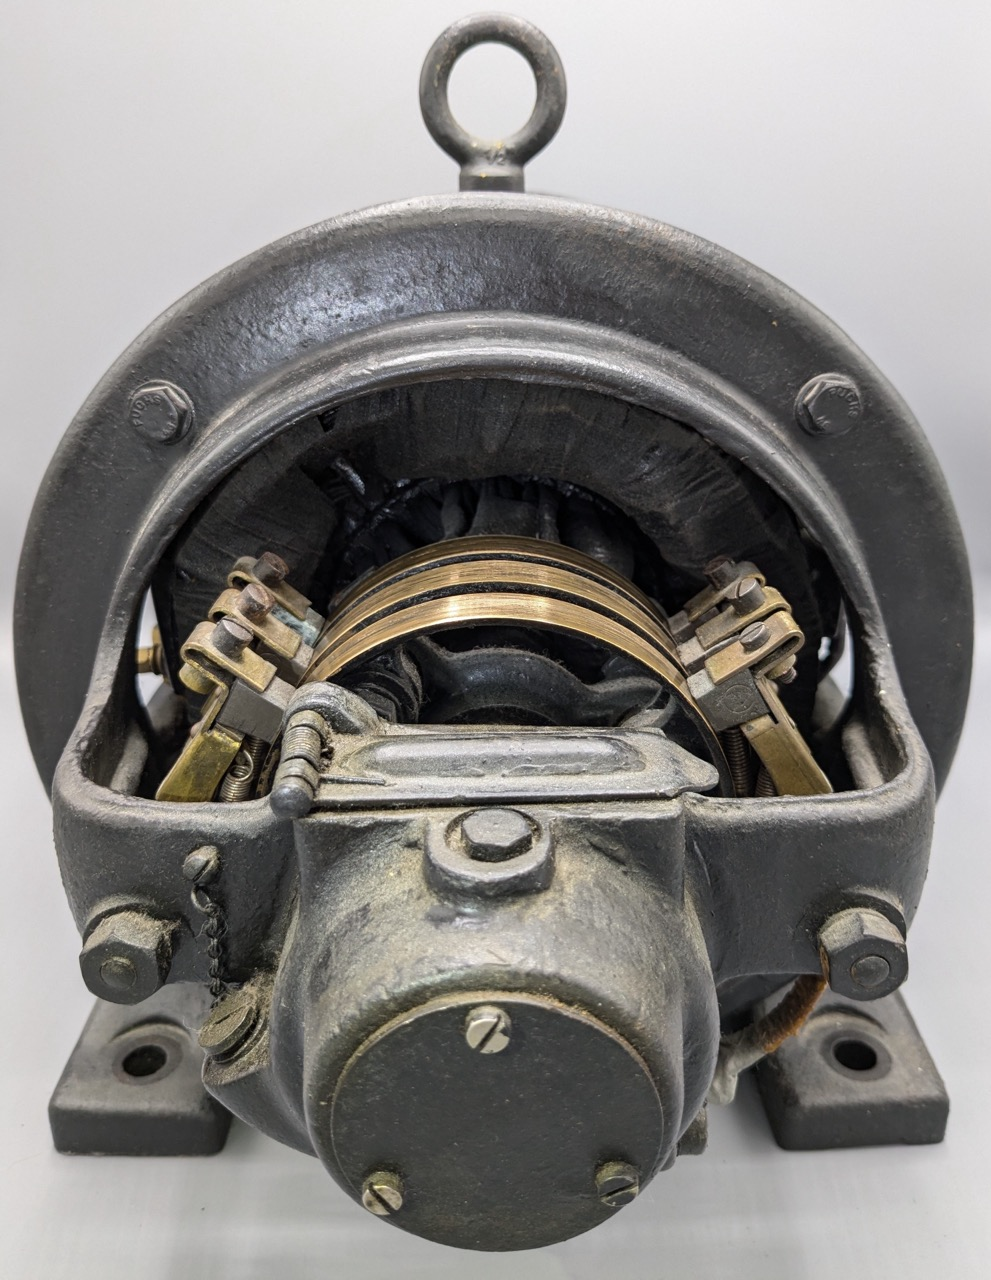
\includegraphics[width=0.5\textwidth]{fig/lec06/Slip_ring_IM.jpg}
			\caption{Wound or \\slip ring rotor}
		\end{subfigure}
        \caption{IM rotor variants} 
        \label{fig:examples_IM_rotor}
	\end{figure}
\end{frame}

%%%%%%%%%%%%%%%%%%%%%%%%%%%%%%%%%%%%%%%%%%%%%%%%%%%%%%%%%%%%%
%% Squirrel cage IM torque-speed characteristic %%
%%%%%%%%%%%%%%%%%%%%%%%%%%%%%%%%%%%%%%%%%%%%%%%%%%%%%%%%%%%%%
\begin{frame}
	\frametitle{Squirrel cage IM torque-speed characteristic} 
    Utilizing the stator flux orientation we define
    $$ \underline{\Psi}_\mathrm{s} = \Psi_\mathrm{s,d} + \mathrm{j}\Psi_\mathrm{s,q} = \Psi_\mathrm{s,d} = \Psi_\mathrm{s}.
    $$
    \pause
    Assuming that the stator ohmic voltage drop is negligible ($R_\mathrm{s}=0$), we get from \eqref{eq:IM_model_voltage_equations_steady_state_slip_ratio} 
    \begin{equation}
        \underline{U}_\mathrm{s} = U_\mathrm{s,d} + \mathrm{j} U_\mathrm{s,q} = \mathrm{j}\omega_\mathrm{s}\underline{\Psi}_\mathrm{s} = \mathrm{j}\omega_\mathrm{s}\Psi_\mathrm{d}
    \end{equation} 
    \pause
    and, therefore,
    \begin{equation}
        U_\mathrm{s,d} = 0, \qquad \Psi_\mathrm{s,d}  = \frac{U_\mathrm{s,q}}{\omega_\mathrm{s}}= \frac{U_\mathrm{s}}{\omega_\mathrm{s}}= \Psi_\mathrm{s}.
        \label{eq:IM_model_stator_flux_orientation_steady_state}
    \end{equation}
    Hence, the stator voltage phasor is purely imaginary and the stator flux phasor is real due to the chosen orientation. \pause From \eqref{eq:IM_model_current_flux_linkage_equations_steady_state} we can rewrite the flux-to-current relationships as
    \begin{equation}
        \begin{split}
            \underline{I}_\mathrm{s} &= \frac{1}{\sigma (L_{\sigma,\mathrm{s}} +M)} \underline{\Psi}_\mathrm{s} -  \frac{M}{\sigma(L_{\sigma,\mathrm{s}} +M)(L'_{\sigma,\mathrm{r}} +M)}\underline{\Psi}'_\mathrm{r},\\
            \underline{I}'_\mathrm{r} &= \frac{1}{\sigma (L'_{\sigma,\mathrm{r}} +M)} \underline{\Psi}'_\mathrm{r} -  \frac{M}{\sigma(L_{\sigma,\mathrm{s}} +M)(L'_{\sigma,\mathrm{r}} +M)}\underline{\Psi}_\mathrm{s}.
        \end{split}
        \label{eq:IM_model_current_flux_linkage_equations_steady_state_squirrel_cage}
    \end{equation}
\end{frame}

%%%%%%%%%%%%%%%%%%%%%%%%%%%%%%%%%%%%%%%%%%%%%%%%%%%%%%%%%%%%%
%% Squirrel cage IM torque-speed characteristic (cont.) %%
%%%%%%%%%%%%%%%%%%%%%%%%%%%%%%%%%%%%%%%%%%%%%%%%%%%%%%%%%%%%%
\begin{frame}
	\frametitle{Squirrel cage IM torque-speed characteristic (cont.)} 
     Furthermore, the rotor voltage for the squirrel cage IM is
     $$
        \underline{U}'_\mathrm{r} = 0
    $$
    due to the short-circuited rotor winding. \pause The rotor voltage equation \eqref{eq:IM_model_voltage_equations_steady_state_slip_ratio} then simplifies to
    \begin{equation}
        0 = \frac{1}{s}R'_\mathrm{r}\underline{I}'_\mathrm{r}+\mathrm{j}\omega_\mathrm{s}\underline{\Psi}'_\mathrm{r} \quad \Leftrightarrow \quad \underline{\Psi}'_\mathrm{r} = \frac{\mathrm{j}}{\omega_\mathrm{s}}\frac{R'_\mathrm{r}}{s}\underline{I}'_\mathrm{r}. 
        \label{eq:IM_model_rotor_flux_steady_state}
    \end{equation}
    \begin{figure}
        \centering
        \includegraphics[width=0.6\textwidth]{fig/lec06/IM_squirrel_T_ECD_steady_state.pdf}
        \caption{T-type ECD of a squirrel cage IM in steady state represented by complex phasors}
        \label{fig:IM_squirrel_T_ECD_steady_state}
    \end{figure}
\end{frame}

%%%%%%%%%%%%%%%%%%%%%%%%%%%%%%%%%%%%%%%%%%%%%%%%%%%%%%%%%%%%%
%% Squirrel cage IM torque-speed characteristic (cont.) %%
%%%%%%%%%%%%%%%%%%%%%%%%%%%%%%%%%%%%%%%%%%%%%%%%%%%%%%%%%%%%%
\begin{frame}
	\frametitle{Squirrel cage IM torque-speed characteristic (cont.)} 
    \onslide<1->
    Combining \eqref{eq:IM_model_stator_flux_orientation_steady_state}, \eqref{eq:IM_model_current_flux_linkage_equations_steady_state_squirrel_cage}, and \eqref{eq:IM_model_rotor_flux_steady_state} we have a linear equation system resulting in 
    \small
    \begin{align}
        \uncover<+->{
        I_\mathrm{s,d} &= \frac{U_\mathrm{s}}{\omega_\mathrm{s}}\frac{\sigma^2 \omega^2_\mathrm{slip} (L_{\sigma,\mathrm{s}} +M)(L'_{\sigma,\mathrm{r}} +M)^3 + (L'_{\sigma,\mathrm{r}} +M)(L_{\sigma,\mathrm{s}} +M)(R'_\mathrm{r})^2 - M^2(R'_\mathrm{r})^2}{\sigma (L_{\sigma,\mathrm{s}} +M)^2(L'_{\sigma,\mathrm{r}} +M) \omega_\mathrm{slip}(\sigma^2 \omega^2_\mathrm{slip}(L'_{\sigma,\mathrm{r}} +M)^2 + (R'_\mathrm{r})^2)},\\}
        \uncover<+->{I_\mathrm{s,q} &= \frac{U_\mathrm{s}}{\omega_\mathrm{s}} \frac{M^2 \omega_\mathrm{slip}R'_\mathrm{r}}{(L_{\sigma,\mathrm{s}} +M)^2(\sigma^2 (L'_{\sigma,\mathrm{r}} +M)^2\omega_\mathrm{slip}^2 + (R'_\mathrm{r})^2)},\\}
        \uncover<+->{I_\mathrm{r,d} &= -\frac{U_\mathrm{s}}{\omega_\mathrm{s}} \frac{\sigma M  \omega_\mathrm{slip}^2(L'_{\sigma,\mathrm{r}} +M)}{(L_{\sigma,\mathrm{s}} +M)(\sigma^2 (L'_{\sigma,\mathrm{r}} +M)^2\omega_\mathrm{slip}^2 + (R'_\mathrm{r})^2)},\\}
        \uncover<+->{I_\mathrm{r,q} &= -\frac{U_\mathrm{s}}{\omega_\mathrm{s}} \frac{M R'_\mathrm{r} \omega_\mathrm{slip}}{(L_{\sigma,\mathrm{s}} +M)(\sigma^2 (L'_{\sigma,\mathrm{r}} +M)^2\omega_\mathrm{slip}^2 + (R'_\mathrm{r})^2)},\\}
        \uncover<+->{\Psi_\mathrm{r,d} &= \frac{U_\mathrm{s}}{\omega_\mathrm{s}}\frac{M (R'_\mathrm{r})^2}{(L_{\sigma,\mathrm{s}} +M) (\sigma^2(L'_{\sigma,\mathrm{r}} +M)^2\omega_\mathrm{slip}^2 + (R'_\mathrm{r})^2)},\\}
        \uncover<+->{\Psi_\mathrm{r,q} &= -\frac{U_\mathrm{s}}{\omega_\mathrm{s}}\frac{\sigma M(L'_{\sigma,\mathrm{r}} +M)R'_\mathrm{r}\omega_\mathrm{slip}}{(L_{\sigma,\mathrm{s}} +M)((L'_{\sigma,\mathrm{r}} +M)^2\sigma^2\omega_\mathrm{slip}^2+(R'_\mathrm{r})^2)}.}
    \end{align}
    \normalsize 
\end{frame}

%%%%%%%%%%%%%%%%%%%%%%%%%%%%%%%%%%%%%%%%%%%%%%%%%%%%%%%%%%%%%
%% Squirrel cage IM torque-speed characteristic (cont.) %%
%%%%%%%%%%%%%%%%%%%%%%%%%%%%%%%%%%%%%%%%%%%%%%%%%%%%%%%%%%%%%
\begin{frame}
	\frametitle{Squirrel cage IM torque-speed characteristic (cont.)} 
    With the definition of $\omega_\mathrm{max}=\nicefrac{R'_\mathrm{r}}{\sigma (L'_{\sigma,\mathrm{r}} +M)}$ we can rewrite and receive \pause
    \small
    \begin{align}
        I_\mathrm{s,d} &= \frac{U_\mathrm{s}}{\omega_\mathrm{s}}\frac{\sigma^2 \omega^2_\mathrm{slip} (L_{\sigma,\mathrm{s}} +M)(L'_{\sigma,\mathrm{r}} +M)^3 + (L'_{\sigma,\mathrm{r}} +M)(L_{\sigma,\mathrm{s}} +M)(R'_\mathrm{r})^2 - M^2(R'_\mathrm{r})^2}{\sigma (L_{\sigma,\mathrm{s}} +M)^2(L'_{\sigma,\mathrm{r}} +M) \omega_\mathrm{slip}(\sigma^2 \omega^2_\mathrm{slip}(L'_{\sigma,\mathrm{r}} +M)^2 + (R'_\mathrm{r})^2)},\\
        I_\mathrm{s,q} &= \frac{U_\mathrm{s}}{\omega_\mathrm{s}}\frac{M^2}{\sigma (L_{\sigma,\mathrm{s}} +M)^2(L'_{\sigma,\mathrm{r}} +M)}\frac{1}{\frac{\omega_\mathrm{slip}}{\omega_\mathrm{max}} + \frac{\omega_\mathrm{max}}{\omega_\mathrm{slip}}},\\
        I_\mathrm{r,d} &= -U_\mathrm{s}\frac{M s}{(L_{\sigma,\mathrm{s}} +M)R'_\mathrm{r}}\frac{1}{\frac{\omega_\mathrm{slip}}{\omega_\mathrm{max}} + \frac{\omega_\mathrm{max}}{\omega_\mathrm{slip}}},\\
        I_\mathrm{r,q} &= -\frac{U_\mathrm{s}}{\omega_\mathrm{s}} \frac{M}{\sigma (L_{\sigma,\mathrm{s}} +M)(L'_{\sigma,\mathrm{r}} +M)}\frac{1}{\frac{\omega_\mathrm{slip}}{\omega_\mathrm{max}} + \frac{\omega_\mathrm{max}}{\omega_\mathrm{slip}}},\\
        \Psi_\mathrm{r,d} &= \frac{U_\mathrm{s}}{\omega_\mathrm{s}}\frac{M R'_\mathrm{r}}{\sigma (L_{\sigma,\mathrm{s}} +M) (L'_{\sigma,\mathrm{r}} +M)\omega_\mathrm{slip}}\frac{1}{\frac{\omega_\mathrm{slip}}{\omega_\mathrm{max}} + \frac{\omega_\mathrm{max}}{\omega_\mathrm{slip}}},\\
        \Psi_\mathrm{r,q} &= -\frac{U_\mathrm{s}}{\omega_\mathrm{s}}\frac{M}{(L_{\sigma,\mathrm{s}} +M)}\frac{1}{\frac{\omega_\mathrm{slip}}{\omega_\mathrm{max}} + \frac{\omega_\mathrm{max}}{\omega_\mathrm{slip}}}.
    \end{align}
    \normalsize 
\end{frame}

%%%%%%%%%%%%%%%%%%%%%%%%%%%%%%%%%%%%%%%%%%%%%%%%%%%%%%%%%%%%%
%% Squirrel cage IM torque-speed characteristic (cont.) %%
%%%%%%%%%%%%%%%%%%%%%%%%%%%%%%%%%%%%%%%%%%%%%%%%%%%%%%%%%%%%%
\begin{frame}
	\frametitle{Squirrel cage IM torque-speed characteristic (cont.)} 
    The torque expression is then
    \begin{equation}
            T = \frac{3}{2} p \sqrt{2}\Psi_\mathrm{s} \sqrt{2}I_\mathrm{s,q} = \frac{3}{2} p \frac{U_\mathrm{s}^2}{\omega_\mathrm{s}^2}\frac{M^2}{\sigma (L_{\sigma,\mathrm{s}} +M)^2(L'_{\sigma,\mathrm{r}} +M)}\frac{2}{\frac{\omega_\mathrm{slip}}{\omega_\mathrm{max}} + \frac{\omega_\mathrm{max}}{\omega_\mathrm{slip}}}.
    \end{equation}
    \pause
    Hence, the maximum achievable torque for a constant stator excitation is
    \begin{equation}
        T_\mathrm{max} = \frac{3}{2} p \frac{U_\mathrm{s}^2}{\omega_\mathrm{s}^2}\frac{M^2}{\sigma (L_{\sigma,\mathrm{s}} +M)^2(L'_{\sigma,\mathrm{r}} +M)}
    \end{equation}
    \pause
    since 
    $$ \max_{\omega_{\mathrm{slip}}} \left\{\frac{2}{\frac{\omega_\mathrm{slip}}{\omega_\mathrm{max}} + \frac{\omega_\mathrm{max}}{\omega_\mathrm{slip}}}\right\} = 1, \qquad \argmax_{\omega_{\mathrm{slip}}} \left\{\frac{2}{\frac{\omega_\mathrm{slip}}{\omega_\mathrm{max}} + \frac{\omega_\mathrm{max}}{\omega_\mathrm{slip}}}\right\} = \omega_\mathrm{max}=\frac{R'_\mathrm{r}}{\sigma (L'_{\sigma,\mathrm{r}} +M)}$$ 
    applies. \pause Above, $\Psi_\mathrm{s}$ and $I_\mathrm{s,q}$ are RMS values according to the complex phasor definitions, which is why the factor $\sqrt{2}$ appears in the torque expression.
\end{frame}

%%%%%%%%%%%%%%%%%%%%%%%%%%%%%%%%%%%%%%%%%%%%%%%%%%%%%%%%%%%%%
%% Squirrel cage IM torque-speed characteristic (cont.) %%
%%%%%%%%%%%%%%%%%%%%%%%%%%%%%%%%%%%%%%%%%%%%%%%%%%%%%%%%%%%%%
\begin{frame}
	\frametitle{Squirrel cage IM torque-speed characteristic (cont.)} 
    The torque expression
    \begin{equation}
        T = T_\mathrm{max} \frac{2}{\frac{\omega_\mathrm{slip}}{\omega_\mathrm{max}} + \frac{\omega_\mathrm{max}}{\omega_\mathrm{slip}}}
    \end{equation}
    can be also alternatively expressed as a function of the slip ratio $s$ \pause by utilizing
    $$
        \omega_\mathrm{slip} = s \omega_\mathrm{s}, \qquad s_\mathrm{max} = \frac{\omega_\mathrm{max}}{\omega_\mathrm{s}} = \frac{R'_\mathrm{r}}{\sigma (L'_{\sigma,\mathrm{r}} +M)\omega_\mathrm{s}}
    $$
    \pause
    leading to
    \begin{equation}
        T = T_\mathrm{max} \frac{2}{\frac{s}{s_\mathrm{max}} + \frac{s_\mathrm{max}}{s}}.
    \end{equation}
    \pause
    The torque-speed characteristic of a squirrel cage IM is also known as Kloss's formula. \pause It should be noted that $\omega_\mathrm{max}$ and $s_\mathrm{max}$ are machine-dependent parameters (for a constant stator excitation), i.e., constants. Contrary, the slip ratio $s$ and slip frequency $\omega_\mathrm{slip}$ depend on the IM's shaft speed and vary during operation.
\end{frame}

%%%%%%%%%%%%%%%%%%%%%%%%%%%%%%%%%%%%%%%%%%%%%%%%%%%%%%%%%%%%%
%% Kloss's formula: visual representation %%
%%%%%%%%%%%%%%%%%%%%%%%%%%%%%%%%%%%%%%%%%%%%%%%%%%%%%%%%%%%%%
\begin{frame}
	\frametitle{Kloss's formula: visual representation}
	\begin{figure}
		\centering
		\begin{subfigure}{0.49\textwidth}
			\centering
			\includegraphics[height=0.65\textheight]{fig/lec06/Kloss_formula_speed.pdf}
			\caption{Illustration based on the mechanical speed}
		\end{subfigure}
		\hfill
		\begin{subfigure}{0.49\textwidth}
			\centering
			\includegraphics[height=0.65\textheight]{fig/lec06/Kloss_formula_slip.pdf}
			\caption{Illustration based on the slip ratio}
		\end{subfigure}
        \caption{Steady-state torque-speed characteristic of a squirrel cage IM for a fixed stator excitation} 
        \label{fig:Kloss_formula}
	\end{figure}
\end{frame}

%%%%%%%%%%%%%%%%%%%%%%%%%%%%%%%%%%%%%%%%%%%%%%%%%%%%%%%%%%%%%
%% Squirrel cage IM torque-speed characteristic: rotor resistance %%
%%%%%%%%%%%%%%%%%%%%%%%%%%%%%%%%%%%%%%%%%%%%%%%%%%%%%%%%%%%%%
\begin{frame}
	\frametitle{Squirrel cage IM torque-speed characteristic: rotor resistance} 
    The starting torque, i.e., the torque at motor standstill ($\omega_\mathrm{r}=0$), is given by
    \begin{equation}
        T_0 = T_\mathrm{max}  \frac{2s_\mathrm{max}}{1+s^2_\mathrm{max}} = T_\mathrm{max}  \frac{2\omega_\mathrm{max}}{1+\omega^2_\mathrm{max}}
    \end{equation}
    since 
    $$\omega_\mathrm{slip} = \omega_{\mathrm{s}} - p \omega_{\mathrm{r}} = \omega_{\mathrm{s}} - 0 = \omega_{\mathrm{s}} $$
    holds. \pause Depending on the machine design $T_0$ can be significantly lower than $T_\mathrm{max}$, which might be a disadvantage for certain applications. \pause Since
    $$\omega_\mathrm{max}=\frac{R'_\mathrm{r}}{\sigma (L'_{\sigma,\mathrm{r}} +M)}, \qquad s_\mathrm{max} = \frac{R'_\mathrm{r}}{\sigma (L'_{\sigma,\mathrm{r}} +M)\omega_\mathrm{s}} $$
    depend on the rotor resistance $R'_\mathrm{r}$, the starting torque can be modified by changing the rotor resistance, e.g., via a dropping resistor or potentiometer (which would require a slip ring rotor).
\end{frame}

%%%%%%%%%%%%%%%%%%%%%%%%%%%%%%%%%%%%%%%%%%%%%%%%%%%%%%%%%%%%%
%% Squirrel cage IM torque-speed characteristic: rotor resistance %%
%%%%%%%%%%%%%%%%%%%%%%%%%%%%%%%%%%%%%%%%%%%%%%%%%%%%%%%%%%%%%
\begin{frame}
	\frametitle{Squirrel cage IM torque-speed characteristic: rotor resistance (cont.)} 
    \begin{figure}
        \centering
        \includegraphics[height=0.65\textheight]{fig/lec06/Kloss_formula_starting_torque.pdf}
        \caption{Steady-state torque-speed characteristic of a squirrel cage IM for a fixed stator excitation with varying rotor resistance $R'_\mathrm{r}$ -- note that the synchronous speed $\omega_\mathrm{r}=\omega_\mathrm{s}/p$ and the maximum torque $T_\mathrm{max}$ are independent of the rotor resistance variation}
        \label{fig:Kloss_formula_starting_torque}
    \end{figure}
\end{frame}

%%%%%%%%%%%%%%%%%%%%%%%%%%%%%%%%%%%%%%%%%%%%%%%%%%%%%%%%%%%%%
%% Slip frequency-dependent rotor skin effect%%
%%%%%%%%%%%%%%%%%%%%%%%%%%%%%%%%%%%%%%%%%%%%%%%%%%%%%%%%%%%%%
\begin{frame}
	\frametitle{Slip frequency-dependent rotor skin effect}
    \begin{columns}
		\begin{column}{0.55\textwidth}
	      \begin{itemize}
            \item<1-> If $\omega_\mathrm{slip} \neq 0$, the rotor bars are exposed to a time-varying magnetic field.
            \item<2-> This induces eddy currents leading to an uneven current distribution within the bars.
            \item<3-> As a result, the effective rotor resistance increases with the slip frequency: \begin{equation}
                \frac{R_\mathrm{r}(\omega_\mathrm{slip})}{R_\mathrm{r,DC}} =  \delta \frac{\sinh(2 \delta) + \sin(2 \delta)}{\cosh(2\delta)-\cos(2 \delta)}
              \end{equation}
              with $$\delta = h_\mathrm{bar}\sqrt{\omega_\mathrm{slip} \frac{\mu_0 \kappa}{2}\frac{w_\mathrm{bar}}{w_\mathrm{slot}}}$$ being the skin depth. Here, $\mu_0$ is the vacuum permeability and $\kappa$ is the bar's conductivity.
          \end{itemize}
        \end{column}
        \begin{column}{0.45\textwidth}
            \onslide<1->
            \begin{figure}
                \centering
                \includegraphics[width=0.85\textwidth]{fig/lec06/Eddy_currents_rotor_bar.pdf}
                \caption{Rotor bar with eddy currents induced by the rotating magnetic field (inspired from A. Binder, \textit{Elektrische Maschinen und Antriebe}, Vol. 2, Springer, 2017)}
                \label{fig:Eddy_currents_rotor_bar}
            \end{figure}
        \end{column}
    \end{columns}
\end{frame}

%%%%%%%%%%%%%%%%%%%%%%%%%%%%%%%%%%%%%%%%%%%%%%%%%%%%%%%%%%%%%
%% Slip frequency-dependent rotor skin effect (cont.)%%
%%%%%%%%%%%%%%%%%%%%%%%%%%%%%%%%%%%%%%%%%%%%%%%%%%%%%%%%%%%%%
\begin{frame}
	\frametitle{Slip frequency-dependent rotor skin effect (cont.)}
    \begin{figure}
        \centering
        \includegraphics[width=0.75\textwidth]{fig/lec06/AC_rotor_resistance.pdf}
        \caption{Rotor resistance of a squirrel cage IM as a function of the slip frequency (example based on the following values: $\kappa = \SI{3.7e7}{\siemens\per\metre}$, $h_\mathrm{bar} = \SI{50}{\milli\metre}$, $w_\mathrm{bar} = \SI{10}{\milli\metre}$, $w_\mathrm{slot} = \SI{15}{\milli\metre}$)}
        \label{fig:AC_rotor_resistance}
    \end{figure}
\end{frame}

%%%%%%%%%%%%%%%%%%%%%%%%%%%%%%%%%%%%%%%%%%%%%%%%%%%%%%%%%%%%%
%% Squirrel cage IM torque-speed characteristic: varying stator frequency %%
%%%%%%%%%%%%%%%%%%%%%%%%%%%%%%%%%%%%%%%%%%%%%%%%%%%%%%%%%%%%%
\begin{frame}
	\frametitle{Squirrel cage IM torque-speed characteristic: varying stator frequency}
    \begin{columns}
		\begin{column}{0.5\textwidth}
	      \begin{itemize}
            \item<1-> Adaption of rotor resistance might be technically tricky.
            \item<2-> Alternative: vary stator frequency $\omega_\mathrm{s}$.
            \item<3-> Shift of the torque-speed characteristic along the speed axis, i.e., the synchronous speed $\omega_\mathrm{r}=\omega_\mathrm{s}/p$.
            \item<4-> Allows utilizing $T_\mathrm{max}$ at different speeds (including initial starting torque).
            \item<5-> Requires a variable frequency source, e.g., a power electronic converter.
          \end{itemize}
        \end{column}
        \begin{column}{0.5\textwidth}
            \onslide<2->
            \begin{figure}
                \centering
                \includegraphics[width=0.95\textwidth]{fig/lec06/Kloss_formula_different_excitation_frequencies.pdf}
                \caption{Steady-state torque-speed characteristic of a squirrel cage IM with varying $\omega_\mathrm{s}$ while keeping $U_\mathrm{s}/\omega_\mathrm{s}=\mathrm{const.}$}
                \label{fig:Kloss_formula_different_excitation_frequencies}
            \end{figure}
        \end{column}
    \end{columns}
\end{frame}

%%%%%%%%%%%%%%%%%%%%%%%%%%%%%%%%%%%%%%%%%%%%%%%%%%%%%%%%%%%%%
%% Squirrel cage IM torque-speed characteristic: flux weakening %%
%%%%%%%%%%%%%%%%%%%%%%%%%%%%%%%%%%%%%%%%%%%%%%%%%%%%%%%%%%%%%
\begin{frame}
	\frametitle{Squirrel cage IM torque-speed characteristic: flux weakening}
    \begin{columns}
		\begin{column}{0.5\textwidth}
	      \begin{itemize}
            \item<1-> The previous consideration from \figref{fig:Kloss_formula_different_excitation_frequencies} assumed that $U_\mathrm{s}/\omega_\mathrm{s}=\mathrm{const.}$ applies, that is, the stator voltage amplitude is adjusted according to the frequency.
            \item<2-> Obviously, this is only possible to a certain extent due to the voltage source limitations.
            \item<3-> Hence, at some point, the torque-speed characteristic is limited by the available voltage leading to a flux weakening operation mode (cf. right figure).
          \end{itemize}
        \end{column}
        \begin{column}{0.5\textwidth}
            \onslide<3->
            \begin{figure}
                \centering
                \includegraphics[width=0.95\textwidth]{fig/lec06/Kloss_formula_different_excitation_frequencies_field_weakening.pdf}
                \caption{Steady-state torque-speed characteristic of a squirrel cage IM with varying $\omega_\mathrm{s}$ while keeping $U_\mathrm{s}=\mathrm{const.}$, i.e., field weakening operation ($\Psi_\mathrm{s}\sim 1/\omega_\mathrm{s}$)} 
                \label{fig:Kloss_formula_different_excitation_frequencies_field_weakening}
            \end{figure}
        \end{column}
    \end{columns}
\end{frame}

%%%%%%%%%%%%%%%%%%%%%%%%%%%%%%%%%%%%%%%%%%%%%%%%%%%%%%%%%%%%%
%% Squirrel cage IM torque-speed characteristic: flux weakening %%
%%%%%%%%%%%%%%%%%%%%%%%%%%%%%%%%%%%%%%%%%%%%%%%%%%%%%%%%%%%%%
\begin{frame}
	\frametitle{Squirrel cage IM torque-speed characteristic: air gap harmonics}
    \begin{columns}
		\begin{column}{0.45\textwidth}
	      \begin{itemize}
            \onslide<1->
            \item The rotating field analysis \eqref{eq:B_three_phase_stator_coil_fourier_series_resulting_field} revealed that the air gap magnetic field contains harmonics:
          \end{itemize}
          $$
          B = \frac{6}{\pi p} \hat{B} \sum_{k}^{\infty} \frac{1}{k} \sin\left(\frac{k \pi}{2}\right) \cos(\omega t - k \vartheta_\mathrm{el}) 
          $$
          \onslide<2->
          \begin{itemize}
            \item This induces rotor currents with the harmonic slip frequency $\omega^{(k)}_\mathrm{slip}$.
            \onslide<3->
            \item Likewise the IM fundamental torque, these air gap field and rotor current harmonics lead to constant, i.e., non-harmonic, torque contributions distorting the torque-speed characteristic.
          \end{itemize}
        \end{column}
        \begin{column}{0.555\textwidth}
            \onslide<3->
            \begin{figure}
                \centering
                \includegraphics[width=0.95\textwidth]{fig/lec06/Kloss_formula_harmonics.pdf}
                \caption{Steady-state torque-speed characteristic of a squirrel cage IM considering torque harmonics due to stator magnetic field harmonics of order $k=1,-5,7,-11$} 
                \label{fig:Kloss_formula_harmonics}
            \end{figure}
        \end{column}
    \end{columns}
\end{frame}